\documentclass[12pt,]{article}
\usepackage{lmodern}
\usepackage{amssymb,amsmath}
\usepackage{ifxetex,ifluatex}
\usepackage{fixltx2e} % provides \textsubscript
\ifnum 0\ifxetex 1\fi\ifluatex 1\fi=0 % if pdftex
  \usepackage[T1]{fontenc}
  \usepackage[utf8]{inputenc}
\else % if luatex or xelatex
  \ifxetex
    \usepackage{mathspec}
  \else
    \usepackage{fontspec}
  \fi
  \defaultfontfeatures{Ligatures=TeX,Scale=MatchLowercase}
\fi
% use upquote if available, for straight quotes in verbatim environments
\IfFileExists{upquote.sty}{\usepackage{upquote}}{}
% use microtype if available
\IfFileExists{microtype.sty}{%
\usepackage{microtype}
\UseMicrotypeSet[protrusion]{basicmath} % disable protrusion for tt fonts
}{}
\usepackage[margin=1in]{geometry}
\usepackage{hyperref}
\hypersetup{unicode=true,
            pdftitle={Einkommensverteilung in Dänemark},
            pdfauthor={Daniel Rosenlechner \& Ingrid Setz},
            pdfkeywords={Dänemark, Einkommensverteilung, Armut, soziale Eingliederung},
            pdfborder={0 0 0},
            breaklinks=true}
\urlstyle{same}  % don't use monospace font for urls
\usepackage{longtable,booktabs}
\usepackage{graphicx,grffile}
\makeatletter
\def\maxwidth{\ifdim\Gin@nat@width>\linewidth\linewidth\else\Gin@nat@width\fi}
\def\maxheight{\ifdim\Gin@nat@height>\textheight\textheight\else\Gin@nat@height\fi}
\makeatother
% Scale images if necessary, so that they will not overflow the page
% margins by default, and it is still possible to overwrite the defaults
% using explicit options in \includegraphics[width, height, ...]{}
\setkeys{Gin}{width=\maxwidth,height=\maxheight,keepaspectratio}
\IfFileExists{parskip.sty}{%
\usepackage{parskip}
}{% else
\setlength{\parindent}{0pt}
\setlength{\parskip}{6pt plus 2pt minus 1pt}
}
\setlength{\emergencystretch}{3em}  % prevent overfull lines
\providecommand{\tightlist}{%
  \setlength{\itemsep}{0pt}\setlength{\parskip}{0pt}}
\setcounter{secnumdepth}{0}
% Redefines (sub)paragraphs to behave more like sections
\ifx\paragraph\undefined\else
\let\oldparagraph\paragraph
\renewcommand{\paragraph}[1]{\oldparagraph{#1}\mbox{}}
\fi
\ifx\subparagraph\undefined\else
\let\oldsubparagraph\subparagraph
\renewcommand{\subparagraph}[1]{\oldsubparagraph{#1}\mbox{}}
\fi

%%% Use protect on footnotes to avoid problems with footnotes in titles
\let\rmarkdownfootnote\footnote%
\def\footnote{\protect\rmarkdownfootnote}

%%% Change title format to be more compact
\usepackage{titling}

% Create subtitle command for use in maketitle
\newcommand{\subtitle}[1]{
  \posttitle{
    \begin{center}\large#1\end{center}
    }
}

\setlength{\droptitle}{-2em}

  \title{Einkommensverteilung in Dänemark}
    \pretitle{\vspace{\droptitle}\centering\huge}
  \posttitle{\par}
  \subtitle{Ökonomie der Verteilung}
  \author{Daniel Rosenlechner \& Ingrid Setz}
    \preauthor{\centering\large\emph}
  \postauthor{\par}
      \predate{\centering\large\emph}
  \postdate{\par}
    \date{22 Februar, 2019}

% Used for placing figures more precisely
\usepackage{float} 
      \let\origfigure\figure 
      \let\endorigfigure\endfigure
      \renewenvironment{figure}[1][2] {
        \expandafter\origfigure\expandafter[H]
      } {\endorigfigure}

\begin{document}
\maketitle
\begin{abstract}
Seit der Jahrhundertwende haben Einkommensverteilung und
Einkommensungleichheit in der Forschung zunehmend an Bedeutung gewonnen,
nicht zuletzt angetrieben durch die Folgen der Finanzkrise. Dänemark
wird oft als Land dargestellt, dass Wirtschaftlichkeit und soziale
Sicherheit erfolgreich im \emph{dänischen Model} umsetzt. Im Rahmen
dieser Arbeit wird die Entwicklung der Einkommensverteilung und in
diesem Zusammenhang Armut und sozialer Ausgrenzung, basierend auf einer
Auswertung von \emph{EU-SILC} Daten, sichtbar gemacht. Die Ergebnisse
zeigen, dass\ldots{}\textbf{WEITERSCHREIBEN}
\end{abstract}

\newpage 

\tableofcontents
\newpage  \listoffigures
\listoftables
\newpage

\newpage

\section{1 Einführung}\label{einfuhrung}

Die Strategie \emph{Europa 2020} ist die Agenda der Europäischen Union
zur Förderung von Wachstum und Beschäftigung des gegenwärtigen
Jahrzehntes. Zu der Umsetzung dieses geimsamen europäischen Vorhaben
wurden in den Bereichen Beschäftigung, Forschung, Klimawandel, Armut und
soziale Ausgrenzung nationale Ziele festgelegt, die jährlich im Rahmen
von Fortschrittsberichten beobachtet werden. Insbesondere soll durch
eine Verringerung der Armut, die soziale Eingliederung gefördert werden,
wobei angestrebt wird, mindestens 20 Millionen Menschen vor dem Risiko
der Armut zu bewahren (Statistisches Amt Europäische Kommission 2016).

Im Rahmen dieser Vorhaben setzt die Europäische Union ein klares Zeichen
zur Bekämpfung von Armut. Während Armut per se sich nur auf den
untersten Teil der Einkommensverteilung bezieht, zeigt die
Einkommensverteilung das Bild der gesamten betrachteten Volkswirtschaft.
Seit der Jahrhundertwende haben Einkommensverteilung und
Einkommensungleichheit in der Forschung zunehmend an Bedeutung gewonnen,
nicht zuletzt angetrieben durch die Folgen der Finanzkrise. Die OECD
weist bereits seit mehreren Jahren auf die Spreizung der Einkommen hin
(OECD 2008; OECD 2015). In dem Report \emph{Growing unequal? Income
distribution and poverty in OECD countries} befasst sich die
Internationale Organisation mit der Entwicklung der Disparität der
Einkommen von 30 Industriestaaten und zeigt auf, dass mindestens seit
der Mitte der 1980er eine geringe, jedoch kontinuierliche Erhöhung der
Ungleichheit stattgefunden hat. Wird dieser Zeitaum näher betrachtet
stellt sich heraus, dass die jeweiligen Regierungen zwar ihre Ausgaben
und Steuern erhöht haben, um dieser Dynamik entgegenzuwirken, wohingegen
der gewünschte Umverteilungseffekt nur bis Mitte der 1990er Jahre
gedämpft werden konnte. In den darauf folgenden Jahren richtete sich die
Umverteilungspolitik weniger gezielt auf ärmere Haushalte und führte zu
einem wesentlich Anstieg der Ungleichheit. Es wird darauf hingewiesen,
dass dies unter anderem ausschlaggebend für die unteschiedlichen
Ausprägungen von Ungleichheit in den jeweiligen Ländern sei (OECD 2008).

Ersichtlich ist, dass eine effiziente nationale Politik Disparitäten
entgegensteuern kann und Steuern und Transfers wichtige Säulen der
Umverteilung sind. Dänemark wird oft als Land dargestellt, dass
Wirtschaftlichkeit und soziale Sicherheit erfolgreich umsetzt. Hier
stellt sich die Frage, ob sich das dänische Model des Wohlfahrtsstaates
auch in der nationalen Einkommensverteilung widerspiegelt. Um die
Einkommensungleichheit und in diesem Zusammenhang die Entwicklung von
Armut und sozialer Ausgrenzung in Dänemark sichtbar zu machen, wird eine
beurteilende Analyse verschiedener Indikatoren auf Basis von
ausgewählten Daten aus der \emph{European Union Statistics on Income and
Living Conditions} (EU-SILC) Erhebung im Rahmen dieses Artikels
vorgenommen.

Der erste Teil beschäftigt sich mit den institutionellen und
theoretischen Grundlagen des Landes und ermöglicht es die Auswertung der
Indikatoren in einen Kontext zu betrachten. Behandelt wird in diesem Zug
der dänische Arbeitsmarkt und das \emph{Flexicurity Prinzip} sowie
Migration und die Folgen der Finanzkrise. Diese Einflussfaktoren sollen
zu einem besseren Verständnis der länderspezifischen Ungleichheit
Dänemarks beitragen. Im Rahmen von Europa 2020 wird anschließend der
Fokus auf das Thema Armut und soziale Ausgrenzung gerückt. Das Kapitel
Methodik befasst sich zum einen auf der Herkunft der verwendeten Daten
und deren Aufbereitung sowie den verschiedenen Einkommenskonzepten, die
zur Analyse herangezogen werden. Außerdem werden hier die Varianten der
Zuteilung von Einkommenskomponenten auf die Haushaltsmitglieder
thematisiert. Die berechneten Indikatoren in Kapitel 5 geben Auschluss
über die Einkommensungleichheit und in wie weit sich Dänemark dem Ziel
der Armutsbekämpfung von der Strategie Europa 2020 bewegt. Zuletzt,
werden alle Erkenntnisse und Ergebnisse im Rahmen des Conclusios
reflektiert und zusammengefasst.

\section{2 Institutionelle und theoretische
Grundlagen}\label{institutionelle-und-theoretische-grundlagen}

Innerhalb der OECD Länder zählt Dänemark traditionell zu den
gleichberechtigteren Ländern und konnte im Jahr 2000 den niedrigsten
Gini-Koeffizienten aller Länder aufweisen (Atkinson 2016). Die
Ungleichheit hat jedoch in den letzten Jahrzehnten zugenommen. Zwar ist
in dem direkten Länder Vergleich die Ungleichheit in Dänemark seit den
1990er Jahren schneller gestiegen, dennoch ist sie auf einem sehr
niedrigen Niveau (OECD 2019a). Zudem hat das Wachstum des
Bruttoinlandproduktes in letzter Zeit dazu beigetragen, dass die obere
Hälfte der Verteilung davon relativ mehr profitierte und die
Umverteilungsmerkmale des Wohlfahrtssystems geschwächt wurden. Dies
bestätigt auch der viel stärkere Anstieg der \emph{Top Incomes} im
Vergleich zu den anderen Dezilen (Causa, Nicolas Ruiz, and Zuzana
Smidova 2016). Veränderte Haushaltsstukturen, wie im besonderen mehr
Studenten und Single-Haushalte, steigende Einwanderung und Alterung
werden als Ursachen für einen großen Teil des Anstiegs genannt (Robling
2018). In einer Analyse aus dem Jahr 2016 stellte der Dänische
Wirtschaftsrat fest, dass die zunehmende Ungleichheit in Dänemark auf
mehrere Komponenten zurückzuführen ist: Das Arbeitseinkommen vor Steuern
ist ungleicher verteilt als zuvor, das Kapitaleinkommen hat als Anteil
am Gesamteinkommen zugenommen und es wird weniger stark umverteilt. Dies
ist darauf zurückführend, dass das dänische System der Einkommenssteuern
in den letzten 20 Jahren aufgrund einer Reihe von Steuerreformen weniger
progressiv ausgerichtet worden ist (Dänischer Wirtschaftsrat 2019).

Seit dem Ausbruch der Ölkrise hatte Dänemark mit anhaltend hohen
Arbeitslosenquoten von rund zehn Prozent zu kämpfen. Um dem
gegenzusteuern und die Arbeitslosigkeit nachhaltig zu senken, wurde das
\emph{Flexicurity} System schrittweise seit den 1990er Jahren
implementiert (Björklund 2000). Flexicurity ist ein Schachtelwort aus
Flexibility und Security und ist zum einen durch lockere
Arbeitsschutzgesetze, großzügige Arbeitslosenversicherungen und zum
anderen durch eine aktive Arbeitsmarktpolitik gekennzeichnet. Ein
weiteres Charakteristikum der Flexicurity Politik stellen sogenannte
aktivierende Maßnahmen dar. So haben beispielsweise Arbeitlose innerhalb
von drei Monaten in Zusammenarbeit mit den Behörden einen Aktionsplan
für den beruflichen Wiedereinstieg zu erstellen. Außerdem können
Weiterbildungsprogramme und die Annahme vermittelter Stellen, unter der
Konsequenz einer Kürzung oder sogar Streichung der
Arbeitslosenunterstützung bei Veweigerung, vorgeschrieben werden. Ziel
dieser strikten Maßnahmen ist es die Dauer der Arbeitslosigkeit zu
senken und sicherzustellen, dass die BezieherInnen bereit sind am
Arbeitsmarkt zu partizipieren (Björklund 2000). Zusätzlich zu den
bereits genannten Reformen wurden, im internationalen Vergleich,
großzügige Karenzmodelle ins Leben gerufen (Gaard 2005). Gallen (2019)
zeigen, dass von 1980 bis 2010 die dänischen Arbeitsmärkte weniger
geschlechterspezifisch geworden sind und die \emph{Gender Earnings Gap}
sich in diesem Zeitverlauf deutlich verringert hat. Letzteres beruht
darauf, dass der Anteil des Lohngefälles, welcher durch Unterschiede in
Bildung, Erfahrung, Beruf und Branche von Frauen im Vergleich zu Männern
erklärt wird, seit den achtziger Jahren zurückgegangen ist und eine
Verringerung der \emph{Gender Hours Gap} stattgefunden hat (Gallen
2019). Insgesamt wendet Dänemark rund 1,8\% des BIPs für aktive
Arbeitsmarktpolitik auf und ist somit in diesem Punkt unter den OECD
Staaten führend (OECD 2016a).

In Folge der Finanzkrise hatte Dänemark mit beträchtlichen
wirtschaftlichen Kosten zu kämpfen, da der wirtschaftliche Abschwung von
2007-2009 der schwerste seit dem Zweiten Weltkrieg war (Causa, Nicolas
Ruiz, and Zuzana Smidova 2016). Einige Schätzungen gehen davon aus, dass
der gesamte Produktionsausfall in den fünf Jahren nach dem Ausbruch der
Krise 12 Prozent der Bruttoinlandsproduktion ausmachte (Bohn-Jespersen
2018). Trotz eines starken und anhaltenden Beschäftigungsrückgangs
aufgrund der Rezession, wirkten eine hohe Arbeitsplatzfluktuation und
Lohnanpassungen, sodass eine langfristige und damit strukturelle
Arbeitslosigkeit nicht folgte. Dies zeigt auch eine tiefergehende
Analyse: Die Zahl der von Arbeitslosigkeit Betroffenen war zwar hoch,
jedoch die Dauer nur kurz, was die Auswirkungen auf die Langzeit- und
Jugendarbeitslosigkeit gedämpft hatte. Dies spricht mitunter auch für
das Wirken des Flexicurity Systems. Auch in den letzten Jahren gab es
eine Reihe von Reformen, die es zum Ziel hatten das Arbeitskräfteangebot
und die Beschäftigung, insbesondere durch Maßnahmen für junge und ältere
Menschen sowie MigrantInnen, zu verbessern (Bohn-Jespersen 2018; Causa,
Nicolas Ruiz, and Zuzana Smidova 2016; OECD 2016a). Die Zielsetzung
hierbei entspricht der zu Beginn erwähnten Analyse von Robling (2018).
Insgesamt ist es angesichts der Probleme, die sich aus Jugendlichen und
ZuwanderInnen ergeben, die mit schwachen Qualifikationen in den
Arbeitsmarkt einsteigen, schwierig eine hohe Beschäftigungsquote mit
einer relativ geringen Lohnstreuung zu erhalten. Da sich die meisten
Jugendlichen im Sekundarbereich II, im postsekundären, nicht-tertiären
oder tertiären Bereich einschreiben, besteht die Hauptherausforderung
darin, die Quoten des Abschlusses zu erhöhen, um sicherzustellen, dass
die Bildungsziele auch erreicht werden. Weiters konnte durch eine Reihe
von Reformen, welche eine vorzeitige Möglichkeit der Pensionierung
verschärft und das Rentenalter erhöht haben, die Tragfähigkeit des
Systems, indem der relative Anteil des Lebens, in welchem die Menschen
arbeiten, erhöht wird und so verstärkt zum Wohlfahrtsstaat beigetragen
wird, sichergestellt werden.

Wie bereits angesprochen, ist ein weiterer Einflussfaktor im Kontext der
Einkommensverteilung Migration. Der Flüchtlingszustrom im Jahr 2015
stellt die größte Massenbewegung in Europa seit dem Zweiten Weltkrieg
dar. Mehr als die Hälfte der Ankünfte beantragte Asyl am nördlichsten
Rand des Kontinents: Hauptziel war bei weitem Deutschland, jedoch
erhielt Schweden mehr Asylsuchende in Bezug auf die Bevölkerung. Die
Niederlande, Norwegen und Dänemark nahmen ebenfalls unbedeutende Zahlen
auf. Seit dem Jahr 2000 wurde die dänische Migrationspolitik
restriktiver (Joyce 2018). Nach und nach wurden unterschiedliche Regeln
eingeführt, um die Asylmigration und die Familienzusammenführung
einzuschränken. Die Sozialleistungen für Flüchtlinge wurden ebenfalls
gekürzt. Infolgedessen sank die Zahl der Asylsuchenden in Dänemark.
Dennoch ist anzumerken, dass MigrantInnen eine deutlich niedrigere
Beschäftigungsquote haben und insbesondere weibliche Migrantinnen
stärker von Armbeitslosigkeit betroffen sind. Als Ursache hierfür wird
auch die Ausgestaltung des dänischen Arbeitsmarkt, der durch hohen
Mindestlöhne und eine Struktur die Erwerbsarmut ausschließt
gekennzeichnet ist, genannt (Joyce 2018). Demenstsprechend sind hohe
Qualifikationsanforderungen vorherrschend und niedrig qualifizierte
Arbeitsplätze gelten als Mangelware. Weiters treten Sprachbarrieren,
Probleme bei der Anerkennung ausländischer Bildungsabschlüsse und
möglicherweise Diskriminierung auf dem Arbeitsmarkt verstärkt auf
(Bohn-Jespersen 2018). Charakterisierend für die dänische
Integrationspolitik ist die starke Involvierung von Gemeinden.
Beispielsweise erhalten die Gemeinden für jeden Flüchtenden, der seine
Arbeit oder eine frühzeitige Ausbildung beginnt, zusätzliche Zuschüsse
(Dänisches Ministerium für Flüchtlinge, Einwanderer und Integration
2017; Joyce 2018).

\section{3 Armut und soziale
Eingliederung}\label{armut-und-soziale-eingliederung}

Artikel 25.1 der \emph{Allgemeinen Erklärung der Menschenrechte}
postuliert den Anspruch eines jeden Menschen auf ein soziales
Existenzminimum und ein System der sozialen Sicherheit:

\begin{quote}
``Jeder {[}Mensch{]} hat das Recht auf einen Lebensstandard, der seine
und seiner Familie Gesundheit und Wohl gewährleistet, einschließlich
Nahrung, Kleidung, Wohnung, ärztliche Versorgung und notwendige soziale
Leistungen gewährleistet sowie das Recht auf Sicherheit im Falle von
Arbeitslosigkeit, Krankheit, Invalidität oder Verwitwung, im Alter sowie
bei anderweitigem Verlust seiner Unterhaltsmittel durch unverschuldete
Umstände.'' (Vereine Nationen 1948)
\end{quote}

Insbesondere sind in diesem Kontext Menschen, die über keinen
entsprechenden Lebensstandard verfügen und von Ungleichheit oder Armut
betroffen sind, von Interesse. Die Komplexität des Begriffes Armut
sollte hierbei noch hervorgehoben werden, da dieser sehr vielfältig
konnotiert ist und nicht einheitlich verwendet wird (Bammer 2003).
Monetäre Armut stellt wohl die offensichtlichste Form von Armut dar.
Personen gelten nach EU Definition als monetär arm, wenn ihr Einkommen
nach Sozialleistungen weniger als 60\% des Medians beträgt. Nur monetäre
Armut zu berücksichtigen, wäre jedoch zu kurz gegriffen. Es ist durchaus
denkbar, dass eine Person nicht als monetär arm gilt und dennoch nicht
in der Lage ist, einen gewissen Mindeststandard an materiellem Wohlstand
zu bestreiten. Hierbei spricht man von materieller Deprivation. Konkret
gilt als materiell depriviert, wer vier der folgen Punkte nicht
finanzieren kann: Miete, Betriebskosten, Reparaturen, Kreditraten; sein
oder ihr Zuhause warm zu halten; unerwartete Ausgaben; jeden zweiten Tag
Fleisch, Fisch oder ein anderes proteinreiches Nahrungsmittel zu essen;
einen einwöchigen Urlaub pro Jahr; ein Auto; eine Waschmaschine; einen
Farbfernseher; ein Telefon. Da sich aber auch der Zugang zum
Arbeitsmarkt auf die Möglichkeit zur sozialen Teilhabe auswirkt, werden
ebenso Personen berücksichtigt, welche in einem Haushalt mit sehr
niedriger Erwerbsintensität leben. Als solche bezeichnet man Haushalte,
in denen Personen im erwerbsfähigen Alter weniger als 20\% der
potenziellen Zeit arbeiten (Statistisches Amt Europäische Kommission
2016).

Somit wird ersichtlich, dass die Messung von Armut und sozialer
Ausgrenzung eines mehrdimensionalen Konstruktes bedarf. Gewiss hat das
(monetäre) Einkommen per se einen starken Einfluss auf die
Lebensbedingungen und die Möglichkeit zur sozialen Teilhabe, jedoch
müssen noch weitere Faktoren berücksichtigt werden um ein
differenziertes Bild zu erhalten. Dementsprechend werden im Rahmen der
\emph{Strategie Europa 2020} Personen als von Armut und sozialer
Ausgrenzung gefährdet definiert, wenn sie von einem der folgenden drei
Umstände betroffen sind: Monetäre Armut, soziale Deprivation oder sehr
niedrige Erwerbsintensität (Statistisches Amt Europäische Kommission
2016).

Maßnahmen, welche gegen Armut und Ungleichheit in Dänemark vorzugehen,
orientieren sich vorwiegend an der Strategie Europa 2020, einer
wirtschaftspolitischen Vorgehensweise der Europäischen Union. Diese soll
für eine soziale Marktwirtschaft sowie für nachhaltiges Wachstum und
solide öffentliche Haushalte Sorge tragen. In diesem Zug wurden fünf
Kernziele in den Bereichen Beschäftigung, Forschung, Klimawandel, Armut
und soziale Ausgrenzung festgelegt, welche in den jeweiligen
Mitgliedsstaaten in nationale Reformziele umgesetzt und vom Basisjahr
2008 ausgehend bis zum Zieljahr 2020 erreicht werden sollen
(Statistisches Amt Europäische Kommission 2016). Wie bereits
angesprochen, stellt die Reduktion von Armut und sozialer Ausgrenzung
eines der zentralen Ziele der Strategie Europa 2020 dar. Ziel der EU ist
es, die Zahl der von Armut oder sozialer Ausgrenzung gefährdeten
Personen bis 2020 um 20 Millionen zu senken (Europäische Kommission
2019). Im Jahr 2016 waren in der EU 118 Millionen Personen von Armut
oder sozialer Ausgrenzung betroffen, das entspricht rund einem Viertel
der Bevölkerung. In Dänemark lag dieser Wert bei einer Million, oder
rund 17\% der Bevölkerung (OECD 2019b).

Um den nationalen Besonderheiten gerecht zu werden, können einzelne
Staaten für Europa 2020 besondere Schwerpunkte setzen. Dänemark legt
dabei ein besonderes Augenmerk auf Personen, die in Haushalten mit sehr
niedriger Erwerbsintensität leben und möchte die Zahl dieser bis 2020 um
22.000 senken (Statistisches Amt Europäische Kommission 2016). Im Jahr
2016 lebten noch eine Million der Däninen und Dänen in Haushalten mit
sehr niedriger Erwerbsintensität (Eurostat 2019). Dies ist auch in dem
Sinne des Fexicurity Pronzeps, da darauf abgezielt wird einen möglichst
großen Teil der Bevölkerung in den Arbeitsmarkt zu integrieren. Ein
weiteres konkretes Ziel der Dänischen Regierung, welches im Rahmen von
Europa 2020 gesetzt wurde und eng mit Armut und sozialer Eingliederung
in Verbindung steht, besteht darin die Chancengleichheit in Dänemark zu
erhöhen, um den sozialen Zusammenhalt in der Gesellschaft zu stärken. Zu
diesem Zweck wurde bereits 2001 ein Sozialfonds eingerichtet, der
sozialer Vererbung entgegenwirken und sozial schwache Gruppen
unterstützen soll. Zu diesen Gruppen zählen unter anderem auch Kinder
und Jugendliche in präkerer Lage. Um dieses Ziel zu erreichen plant die
dänische Regierung die Zivilgesellschaft und den Einsatz von
Freiwilligenarbeit zu stärken und finanziell zu unterstützen,
Obdachlosigkeit zu bekämpfen, präzise Armutsindikatoren zu entwickeln,
sowie Strategien in Bezug auf Ghettoisierung und Drogenmissbrauch zu
entwickeln. Diese Maßnahmen werden vom dänischen Sozialfonds finanziert,
in welchen jährlich rund eine Milliarde Dänische Kronen fließen. Das
entspricht rund 130 Millionen Euro oder knapp 5 Prozent des dänischen
Bruttoinlandsprodukts (Dänische Regierung 2010).

Insgesamt ist der Anteil der von Armut oder sozialer Ausgrenzung
betroffenen Personen an der Bevölkerung in Dänemark im internationalen
Vergleich sehr niedrig. Außerdem ist Dänemark sehr erfolgreich darin,
durch Sozialausgaben monetäre Armut zu beseitigen. Dies wird an der
Differenz der Armutsgefährdungsquoten vor und nach Steuern eruiert. In
Dänemark lag dieser Wert 2014 bei knapp 15\%, der EU-weite Wert lag bei
knapp 9\% (Statistisches Amt Europäische Kommission 2016).

\section{4 Methodologie}\label{methodologie}

\subsection{4.1 Daten}\label{daten}

Für eine Analyse liefert die Erhebungen \emph{European Union Statistics
on Income and Living Conditions} (EU-SILC) hinreichend detaillierte
Daten. Ausschließlich für die Inflationsbereinigung werden Daten von dem
\emph{Statistischen Amt der Europäischen Union} (Eurostat) herangezogen.
Erstmals wurde die EU-SILC Erhebung 2003, basierend auf einer
freiwilligen Vereinbarung zwischen Eurostat und sechs EU-Mitgliedstaaten
(Belgien, Dänemark, Griechenland, Irland, Luxemburg und Österreich)
sowie Norwegen durchgeführt. Inzwischen beteiligen sich neben den
EU-Mitgliedsstaaten auch Norwegen, Island, die Türkei, die Schweiz,
Mazedonien und Serbien an der harmonisierten Stichprobenerhebung von
privaten Haushalten (Eurostat 2019). Das Hauptaugenmerk der Erhebung
liegt in der Beobachtung von Armut und sozialer Ausgrenzung und dient in
diesem Kontext zur Überwachung der Strategie Europa 2020.

Generell werden multidimensionale Mikrodaten zu Einkommen, Armut,
sozialer Ausgrenzung, Wohnraum, Arbeit, Bildung und Gesundheit erfasst.
Es handelt sich hierbei zum einen um \emph{Querschnittsdaten} über einen
bestimmten Zeitpunkt und zum anderen \emph{Längsschnittdaten}, welche
Veränderungen auf individueller Ebene über einen gewissen Zeitraum
beobachten (Eurostat 2013a). Anzumerken ist, dass aufgrund der engen
Definition von Haushalten, Personen, die in Anstaltshaushalten oder
Gemeinschaftsunterkünften leben oder ohne festen Wohnsitz sind, nicht in
den Daten erfasst werden.

Wie bereits angeführt, nimmt Dänemark seit der Erstherbung an der
EU-SILC Erhebung teil. Hervorzuheben ist, dass Dänemark sowie die
restlichen nordischen Länder, Holland und Slowenien zu den einzigen
Ländern gehören, in welchen die Einkommensstatistiken auf vollständigen
Registern basieren (Danmarks Statistik 2019b). Die von der nationalen
Statistikbehörde \emph{Danmarks Statistik} durchgeführte
primärstatistische Erhebung wird sowohl mit Hilfe von persönlichen
(\emph{Computer Assisted Personal Interview}) und telefonischen
(\emph{Computer Assisted Telephone Interview}) Interviews als auch
computergestützte (\emph{Computer Assisted Web Interviews})
Webinterviews realisiert. Im Jahr 2012 präsentierte Danmarks Statistik
erstmals seine Erfahrung mit der Verwendung von Computer Assisted Web
Interviews (CAWI) für subjektive Variable im Rahmen von den Erhebungen
(Eurostat 2013b). Für diese Arbeit sind die nach CAWI-erhobenen Daten
jedoch nicht relevant, da diese in der Pilotphase nur die Variablen
PW010, HS120, HS040 und HS060 betreffen (Danmarks Statistik 2014).

\subsection{4.2 Einkommenskonzepte}\label{einkommenskonzepte}

Im Rahmen der Analyse der Einkommensverteilung in Dänemark werden
folgende drei Einkommenskonzepte verwendet, um etwaige Unterschiede in
der Entwicklung der Indikatoren besser zu verfolgen und Rückschlüsse auf
die Herkunft etwaiger Veränderungen der Lebensbedingungen zu ziehen
(detaillierte Beschreibungen der jeweiligen Variablen sind von
\emph{Gesis}\footnote{\url{https://www.gesis.org/en/missy/metadata/EU-SILC/}}
einsehbar):

\textbf{1. Faktoreinkommen vor Steuern} Das vorsteuerliche
Faktoreinkommen setzt sich aus der Summme aus Arbeitseinkommen inklusive
Selbstständiger (PY010G, PY021G, PY050G, HY110G) und Vermögenseinkommen
(HY040G, HY090G, PY080G) zusammen. Dieses Einkommenskonzept erfasst
somit nur die Einkommen aus aktiver Produktion. Unter der Annahme, dass
kein Transfersystem existiert, wird durch die Betrachtung des
vorsteuerlichen Faktoreinkommens eine direkte Verbindung zu den
Arbeitsmärkten geschaffen.

\textbf{2. Nationaleinkommen vor Steuern} Das Nationaleinkommen vor
Steuern inkludiert neben den Komponenten des Faktoreinkommens vor
Steuern noch Pensionen (PY100G) und Arbeitslosengeld (PY090G). In diesem
Einkommenskonzept werden nur arbeitsrelevante Transferzahlungen
hinzugezogen, um eine etwaige Verzerung aufgrund von Veränderungen in
der Altersstrukturen (Personen in Pension mit keinem beziehungsweise
geringem Faktoreinkommen) zu berücksichtigen. Unterschiede in der
Entwicklung von Faktoreinkommen vor Steuern und Nationaleinkommen vor
Steuern legen Reformen im Bereich der Arbeitslosen- beziehungsweise
öffentlichen Pensionsversicherung nahe.

\textbf{3. Verfügbares Einkommen nach Steuern} Das verfügbare Einkommen
nach Steuern inkludiert neben den Komponenten des Nationaleinkommens vor
Steuern alle anderen erhaltenen Transferzahlungen (PY110G, PY120G,
PY130G, PY140G, HY050G, HY060G, HY070G, HY080G) abzüglich aller direkten
Steuern und Sozialversicherungsabgaben (HY120G, HY130G, HY140G).
Schließlich zeigt das verfügbare Einkommen nach Steuern wie der Staat
die Höhe und Verteilung der verfügbaren Einkommen durch (weitere)
monetäre Transfers beeinflussen kann.

Zu beachten ist, dass es über die Jahre zu Änderungen in der Definition
der EU-SILC Daten kam. Dementsprechend ist ein uneingeschränkter
Vergleich zwischen den Jahren nicht möglich, dennoch lassen sich daraus
interessante Entwicklungen ableiten.

\subsection{4.3 Allokation der
Haushaltskomponenten}\label{allokation-der-haushaltskomponenten}

Wie aus den oberen Konzepten erkenntlich, gibt es sowohl Variablen auf
Personen- (PY010G) als auch Haushaltsebene (HY110G). Die
Einkommenskomponenten beziehungsweise Steuern, die nur auf
Haushaltsebene verfügbar sind, werden auf die einzelnen
Haushaltsmitgleider aufgeteilt. Die Allokation erfolgt nach folgenden
zwei Aufschlüsselungsmethoden:

\textbf{1. P1 Eurostat } Hierbei werden alle Einkommen eines Haushaltes
in einem gleichem Maß auf die äquivalten Haushaltsmitglieder aufgeteilt.

\textbf{2. P2 wid.world } Im Gegensatz zu der vorhergehenden Variante,
werden hier nicht mehr alle in einem Haushalt lebenden Personen in das
Sample genommen. Hier erfolgt eine Ausschließung von Personen unter 20
Jahren. Außerdem werden lediglich die Einkommensvariablen, die nur auf
Haushaltsebene verfügbar sind, gleichmäßig durch die Anzahl der
Haushaltsmitglieder (\textgreater{}20) auf alle Haushaltsmitgleider
aufgeteilt; die persönlichen Einkommen bleiben den jeweiligen Personen
vorbehalten.

\section{5 Empirische Analyse}\label{empirische-analyse}

Im Folgenden wird die Einkommensverteilung in Dänemark anhand von
mehreren standardisierten Indikatoren für den Zeitraum 2004-2017
analysiert, um Rückschlüsse über die Ungleichheit des Landes zu geben.
Hierbei ist es von Interesse die verschiedenen Einkommenskonzepte
differenziert zu betrachten und die jeweiligen Veränderungen in der
Verteilung der Einkommen zu beobachten.

In diesem Abschnitt liegt der Fokus der Auswertung auf P1. Begründet
wird dies dadurch, dass die Steuerdaten nur auf Haushaltsebene verfügbar
sind. Würden wir beispielsweise die Variante P2 heranziehen, wenn wir
eine geringverdienende Frau mit sehr gut verdienenden Mann betrachten,
stellt sich heraus, dass sie neben ihrem geringen Einkommen die
Steuerlast ihres Mannes in der Einkommensverteilung mitträgt. Sämtliche
Gesamtübersichten der berechneten Indikatoren befinden sich für beide
Allokationsvarianten, sprich P1 Eurostat und P2 wid.world, im Appendix.

\subsection{5.1 Mittelwert und Median}\label{mittelwert-und-median}

Für einen ersten Eindruck, werden Mittelwert und Median Einkommen näher
betrachtet, da diese Aufschluss über die Schiefe der Verteilungsfunktion
geben. Die Abbildung 1 zeigt die Entwicklung des Median- und
Durchschnittseinkommens nach Steuern (Einkommenskonzept 3) seit 2004.

\begin{figure}
\centering
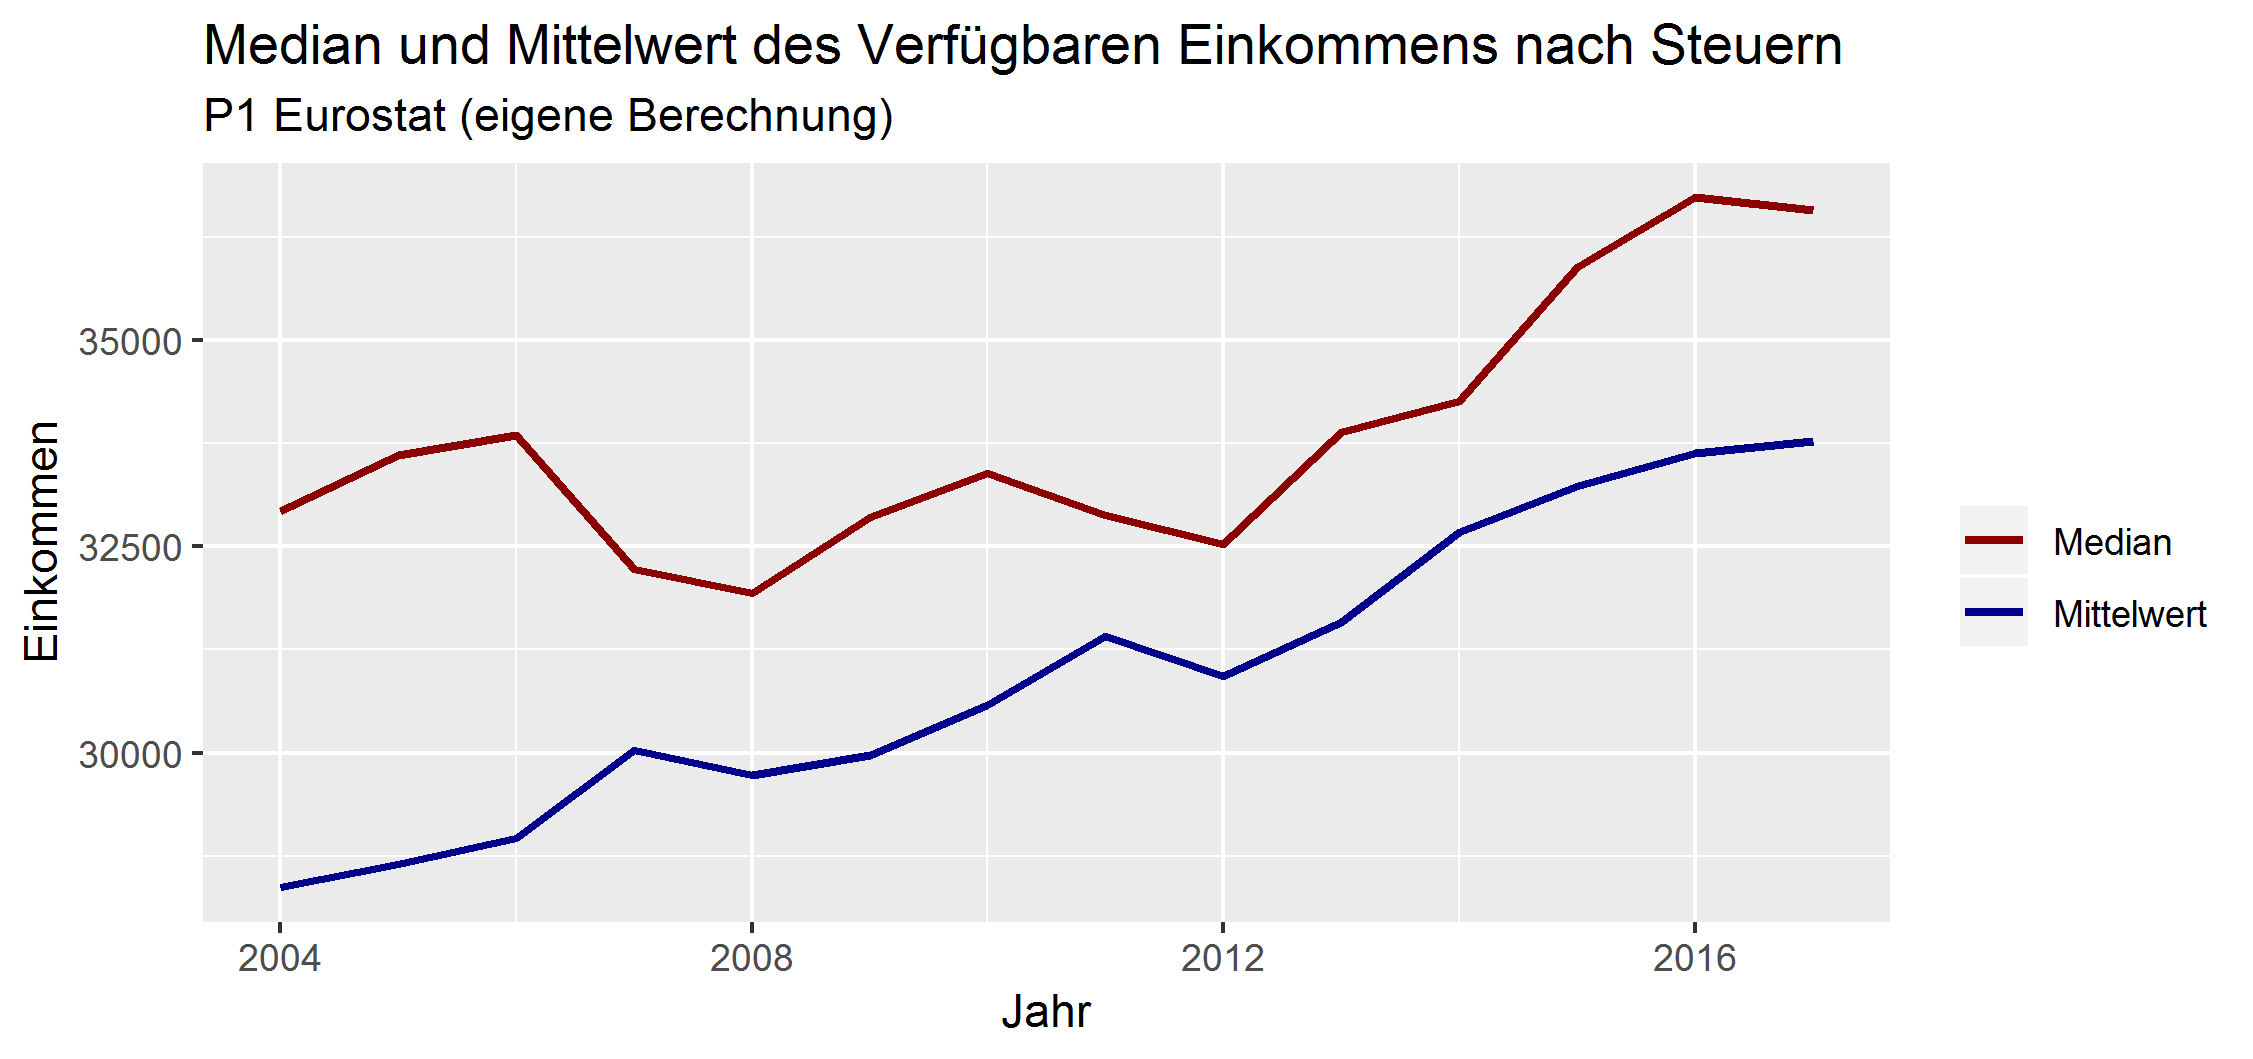
\includegraphics[width=0.65000\textwidth]{img/medmit.png}
\caption{Median und Mittelwert, 2004-2017}
\end{figure}

Es fällt sofort ins Auge, dass beide Werte über den Zeitverlauf stark
gestiegen sind. Die Betrachtung des durchschnittlichen Jahreseinkommen
zeigt von 2004 bis 2017 eine Erhöhung von rund 28.371 DKK auf 33.776
DKK, was knapp 20\% entspricht. Für das Medianeinkommen beträgt die
Erhöhung in diesem Fall lediglich rund 15\%.

Da das Durchschnittseinkommen deutlich unter dem Medianeinkommen liegt,
kann man daraus schließen, dass die Einkommensverteilung eine
rechtsschiefe Dichtefunktion ausweist. Dies ist charakteristisch für
eine Einkommensverteilung. Aus der Grafik ist gut ersichtlich, dass
Dänemark nicht unverschohnt von der Wirtschafts- und Finanzkrise 2008
geblieben ist und sich diese auf die Einkommen privater Haushalte
negativ ausgewirkt hat. Diese Annahme wird durch Danmarks Statistik
(2019a) bestätigt, die auch zeigen, dass Dänemark die Folgen der Krise
langsamer kompensiert hat als dessen Nachbarländer.

\subsection{5.2 Gini Koeffizient}\label{gini-koeffizient}

Durch den Vergleich von Median und Mittelwert lassen sich nur beschränkt
Schlüsse auf die Einkommensverteilung ziehen. Ein detaillierteres Bild
liefert der Gini Koeffizient. Entspricht der Gini einem Wert von Null,
liegt vollständige Gleichverteilung vor, nimmt er 1 an, so gehört einer
Person das ganze Vermögen in der Gesellschaft.

\begin{figure}
\centering
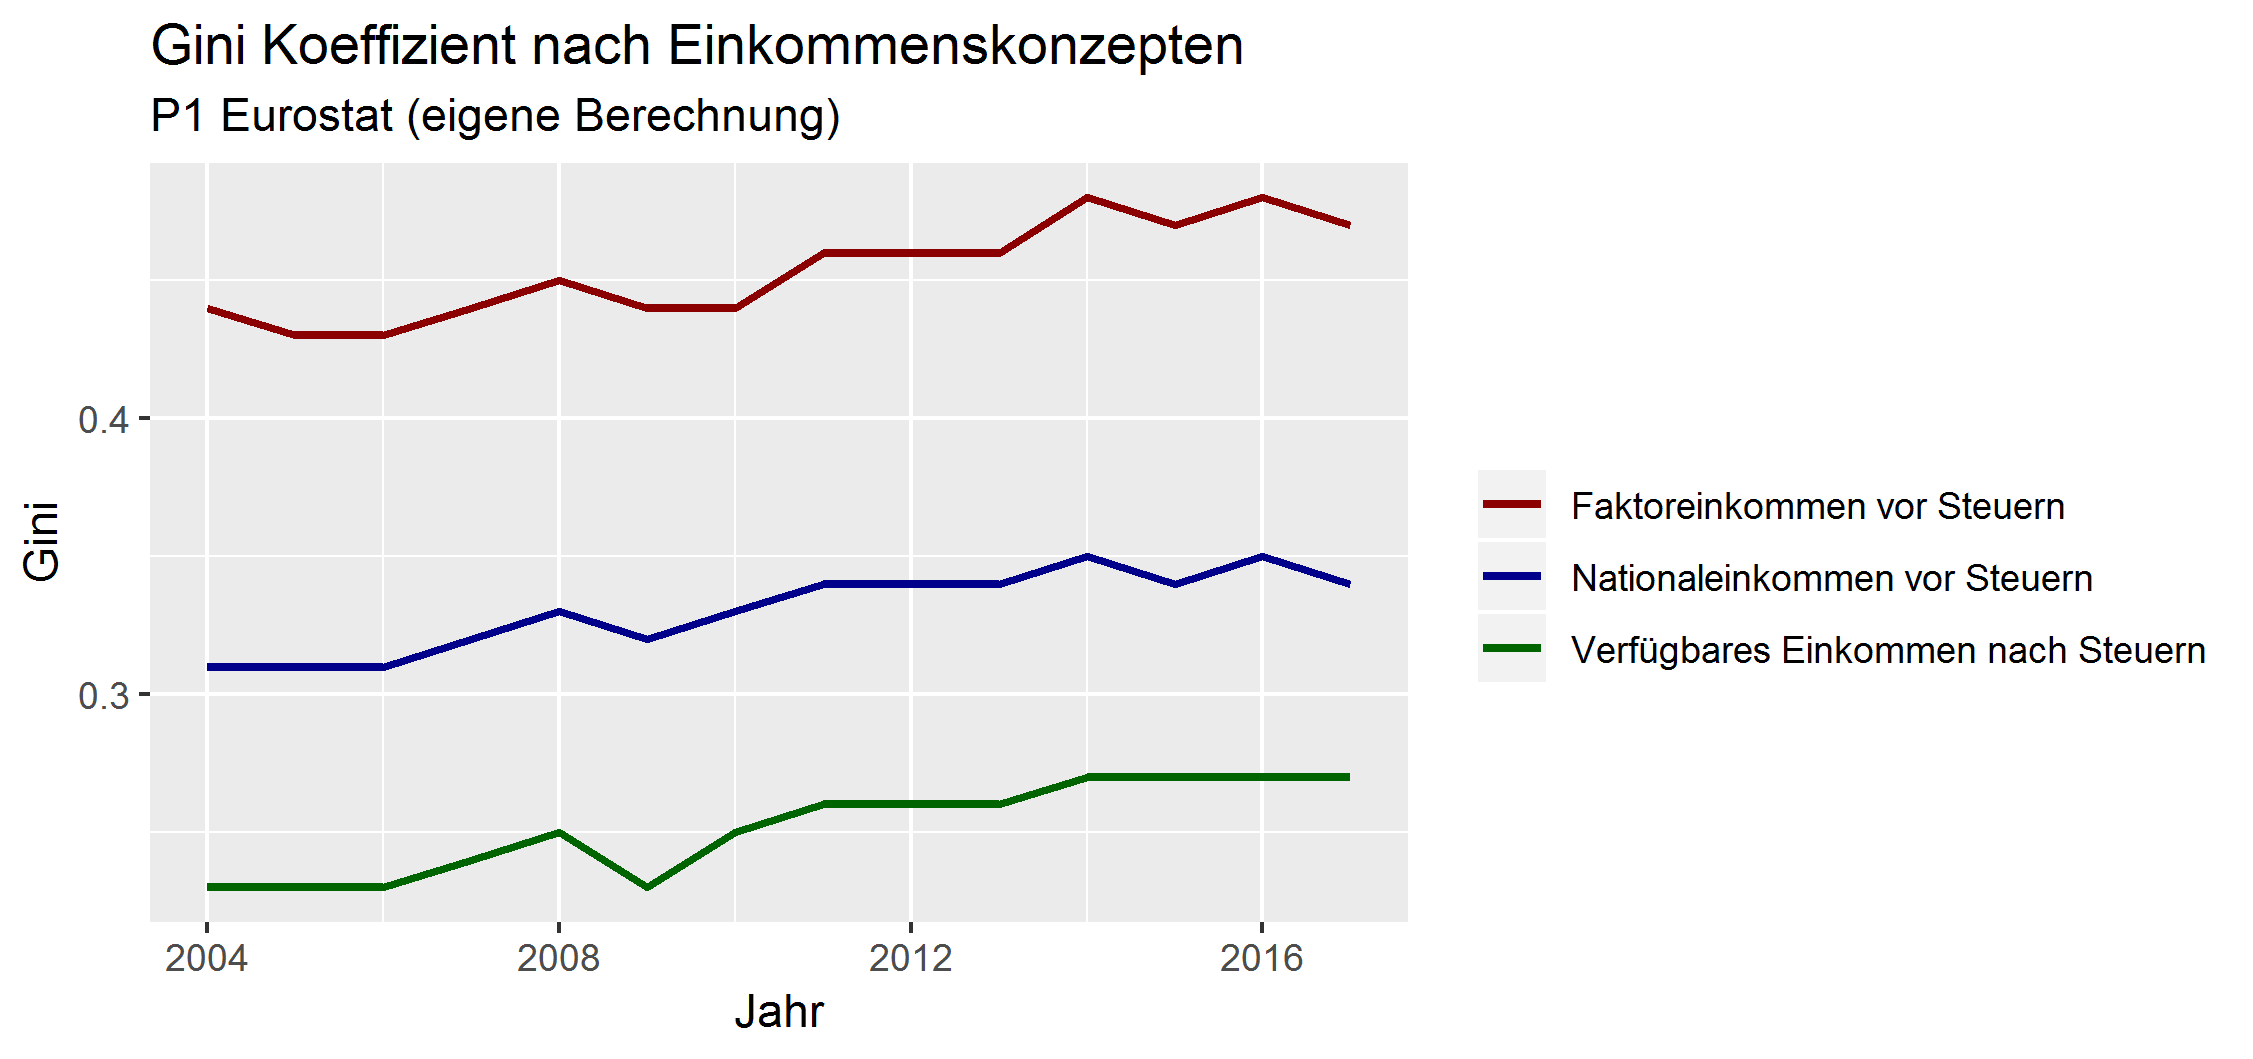
\includegraphics[width=0.65000\textwidth]{img/gini.png}
\caption{Gini-Index, 2004-2017}
\end{figure}

Abbildung 2 zeigt die Entwicklung des Gini Koeffizienten nach den drei
Einkommenskonzepten seit 2004. Klar ersichtlich ist, dass die
staatlichen Umverteilungssysteme die\\
Einkommensungleichheit stark sinken lassen. Dies sieht man beim
Vergleich des Ginis für das verfügbare Einkommen nach Steuern mit den
beiden anderen Einkommenskonzepten. Sowohl Arbeitslosenunterstützung und
Pensionen als auch Steuer- und Transfersysteme lassen die Ungleichheit
in einem größeren Ausmaß sinken. Für das Jahr 2017 bedeutet dies eine
Senkung von insgesamt 20\%. Insgesamt ist im Zeitverlauf die
Ungleichheit in Dänemark gestiegen. Außerdem zeigt Tabelle 5 aus dem
Appendix, dass der Gini-Koeffizient nach der Berechnung P2 für alle
Zeitpunkte deutlich höher ist. Dies erfolgt aus der Konstruktion der
Allokationsvariante.

Lorenzkurve??

\subsection{5.3 P80/P20 Verhältnis}\label{p80p20-verhaltnis}

Das P80/P20 Verhältnis stellt den Mittelwert der oberen 20\% relativ zu
den unteren 20\% der EinkommensbezieherInnen gegenüber.

\begin{figure}
\centering
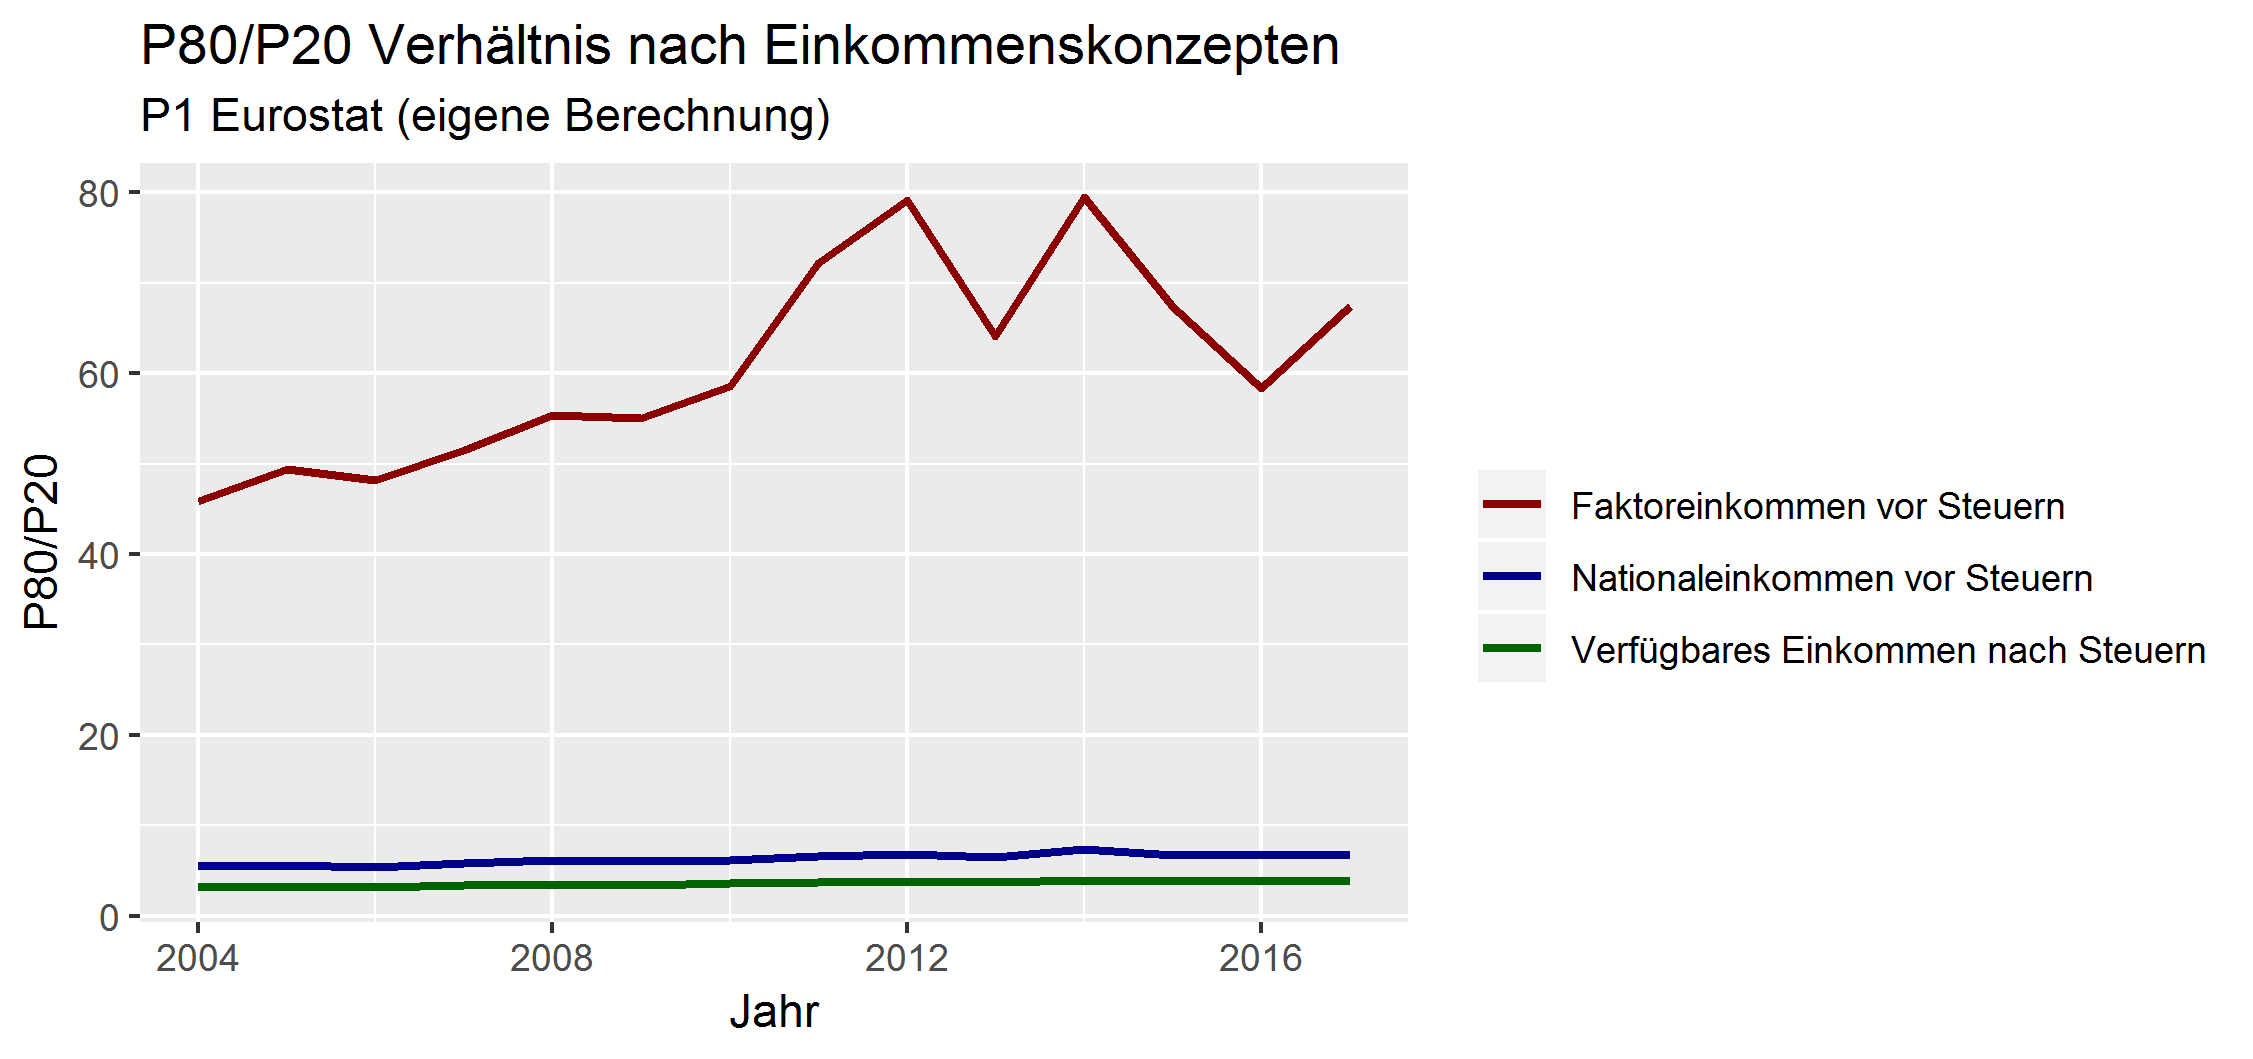
\includegraphics[width=0.65000\textwidth]{img/8020.png}
\caption{P80/P20 Verhältnis, 2004-2017}
\end{figure}

Um das P80/P20 Verhältnis für Dänemark zu illustrieren, werden die drei
verschiedenen Einkommenskonzepte über den Zeitrahmen 2004-2017 in
Abildung 3 betrachtet. Unter der Annahme, dass der mittlere
Einkommensteil in diesem Verhältnis ausgeblendet wird, ist dieses Maß
wesentlich sensitives bei Veränderungen an den Rändern der Verteilung.
Für die Auswertung von Dänemark sieht man, dass der Unterschied zwischen
Faktoreinkommen vor Steuern und dem verfügbaren Einkommen nach Steuern
zu einem größeren Teil durch das progressive Steuersystem erklärbar ist.
Dieses Verteilungsmaß zeigt einen leicht steigenden Trend zu mehr
Ungleichheit. Für die verfügbaren Einkommen beträgt das P80/P20
Verhältnis rund 4\%. Dies bedeutet, dass eine Person aus den top 20\% im
Durchschnitt das vier-fache des Einkommens einer Person der unteren 20\%
verdient.

\subsection{5.4 Top 10\% Anteil}\label{top-10-anteil}

Der Top 10\% Anteil gibt Auskunft ob die Einkommen an der Spitze davon
laufen.

Abbildung 4 zeigt die Entwicklung des Top 10\% Anteils nach den drei
Einkommenskonzepten für beide Allokationsvarianten. Der Anteil der Top
10\% ist für die jeweiligen Einkommenskonzepte im Zeitverlauf konstant.
Für die verfügbaren Einkommen liegt dieser Wert für P1 im Durchschnitt
bei 0,57 und bei P2 0,50. Dies bedeutet, dass die Top-Verdiener die
Hälfte des Gesamteinkommens beziehen. Die Einkommenskonzepte
Nationaleinkommen vor Steuern und das verfügbare Einkommen nach sind in
beiden Varianten P1 und P2, wie zu erwarten, nahezu ident. Da die Werte
der Top-10\% über den Zeitverlauf konstant erscheinen, lässt ich daraus
schließen, dass die Umverteilungslast von anderen Einkommensschichten
getragen wird.

\subsection{5.5 Armutsgefährdungsquote}\label{armutsgefahrdungsquote}

Ein wertvoller Indikator hierbei ist die Armutsgefährdungsquote. Diese
zeigt den Anteil jener, die aufgrund ihres relativ geringen Einkommens
von Armut und sozialer Ausgrenzung bedroht sind. Nach dem EU-Standard
entspricht diese Quote dem Anteil der Personen, deren
Äquivalenzeinkommen weniger als 60\% des Medians der Äquivalenzeinkommen
der Bevölkerung beträgt. Daraus ist ersichtlich, dass die
Armutsgefährdungsquote nur relativ betrachtet werden kann und häufig
(nicht zwanghaft) auf einen niedrigen Lebensstandard der Betroffenen
hindeutet.

Mit Hilfe der oben erwähnten Indikatoren lässt sich zeigen, dass vor
allem das untere Ende der Einkom-mensverteilung durch staatliche
Umverteilung profitiert. Jedoch darf nicht außer Acht gelassen
werden,dass ein signifikanter Teil des untersten Dezils selbst
imPost-tax disposable incomearmutsgefährdet ist.Wir folgen hier der
Eurostat-Definition:

Die Strategie Europa 2020 hat es sich zum Ziel gesetzt, mindestens 20
Millionen Menschen vor dem Risiko der Armut zu bewahren. Dementsprechend
stehen die jeweiligen Staaten mit ihren abgestimmten nationalen
Benchmarks vor einer großen gemeinschaftlichen Herausforderung . Im
folgenden wird analysiert, in wie weit sich Dänemark Richtung dem Ziel
der Armutsbekämpfung von der Strategie Europa 2020 bewegt und ob eine
positive Tendenz erkennbar ist.

\begin{figure}
\centering
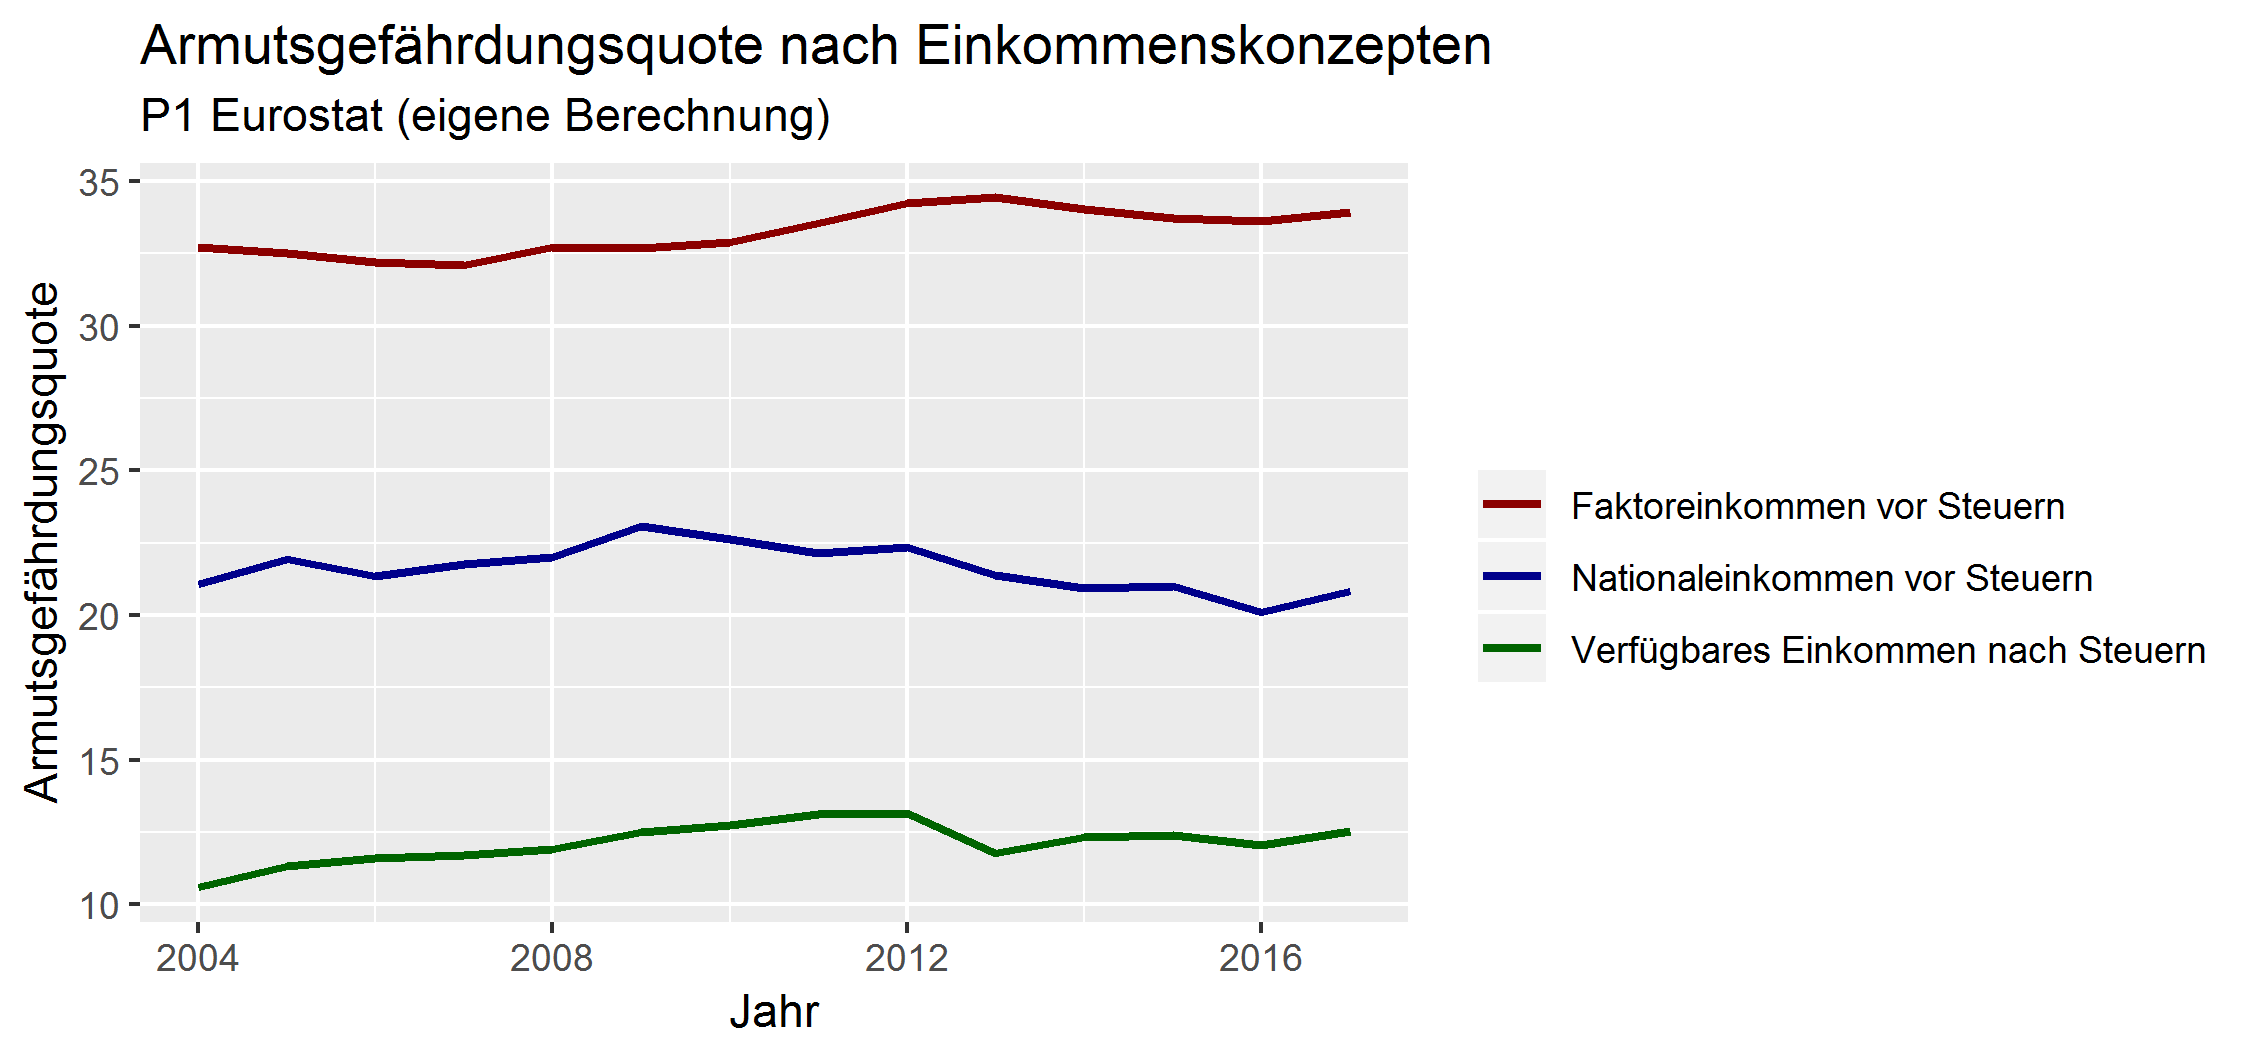
\includegraphics[width=0.90000\textwidth]{img/arpr.png}
\caption{Armutsgefährdungsquote, 2004-2017}
\end{figure}

Abbildung 4 zeigt die Entwicklung der Armutsgefährdungsquote nach den
drei Einkommenskonzepten für P1. Insgesamt ist die
Armutsgefährdungsquote über den Zeitverlauf gestiegen. Unter alleiniger
Betrachtung des verfügbaren Einkommens nach Steuern ist hier ein Anstieg
von 1,95\% in dem Zeitraum 2004-2017 beobachtbar. Zwar kann Dänemark im
EU-Vergleich eine gerine Armutsgefährdungsquote per se aufweisen,
dennoch bewegt sich das Land noch nicht in die richtige Richtung für die
Strategie Europa2020. Dies bedeutet, dass die 2010 von Europäischen Rat
verabschiedeten Zielvorgaben die bis 2020 erfüllt werden sollten, in
weitere Ferne rücken. Vergleichen wir 2010 mit den neuesten Werten von
2017 (im Detail siehe Appendix) ist kaum eine Veränderung der Rate
beobachtbar.

\subsection{5.5.1 Zerlegung der
Armutsgefährdungsquote}\label{zerlegung-der-armutsgefahrdungsquote}

\begin{figure}
\centering
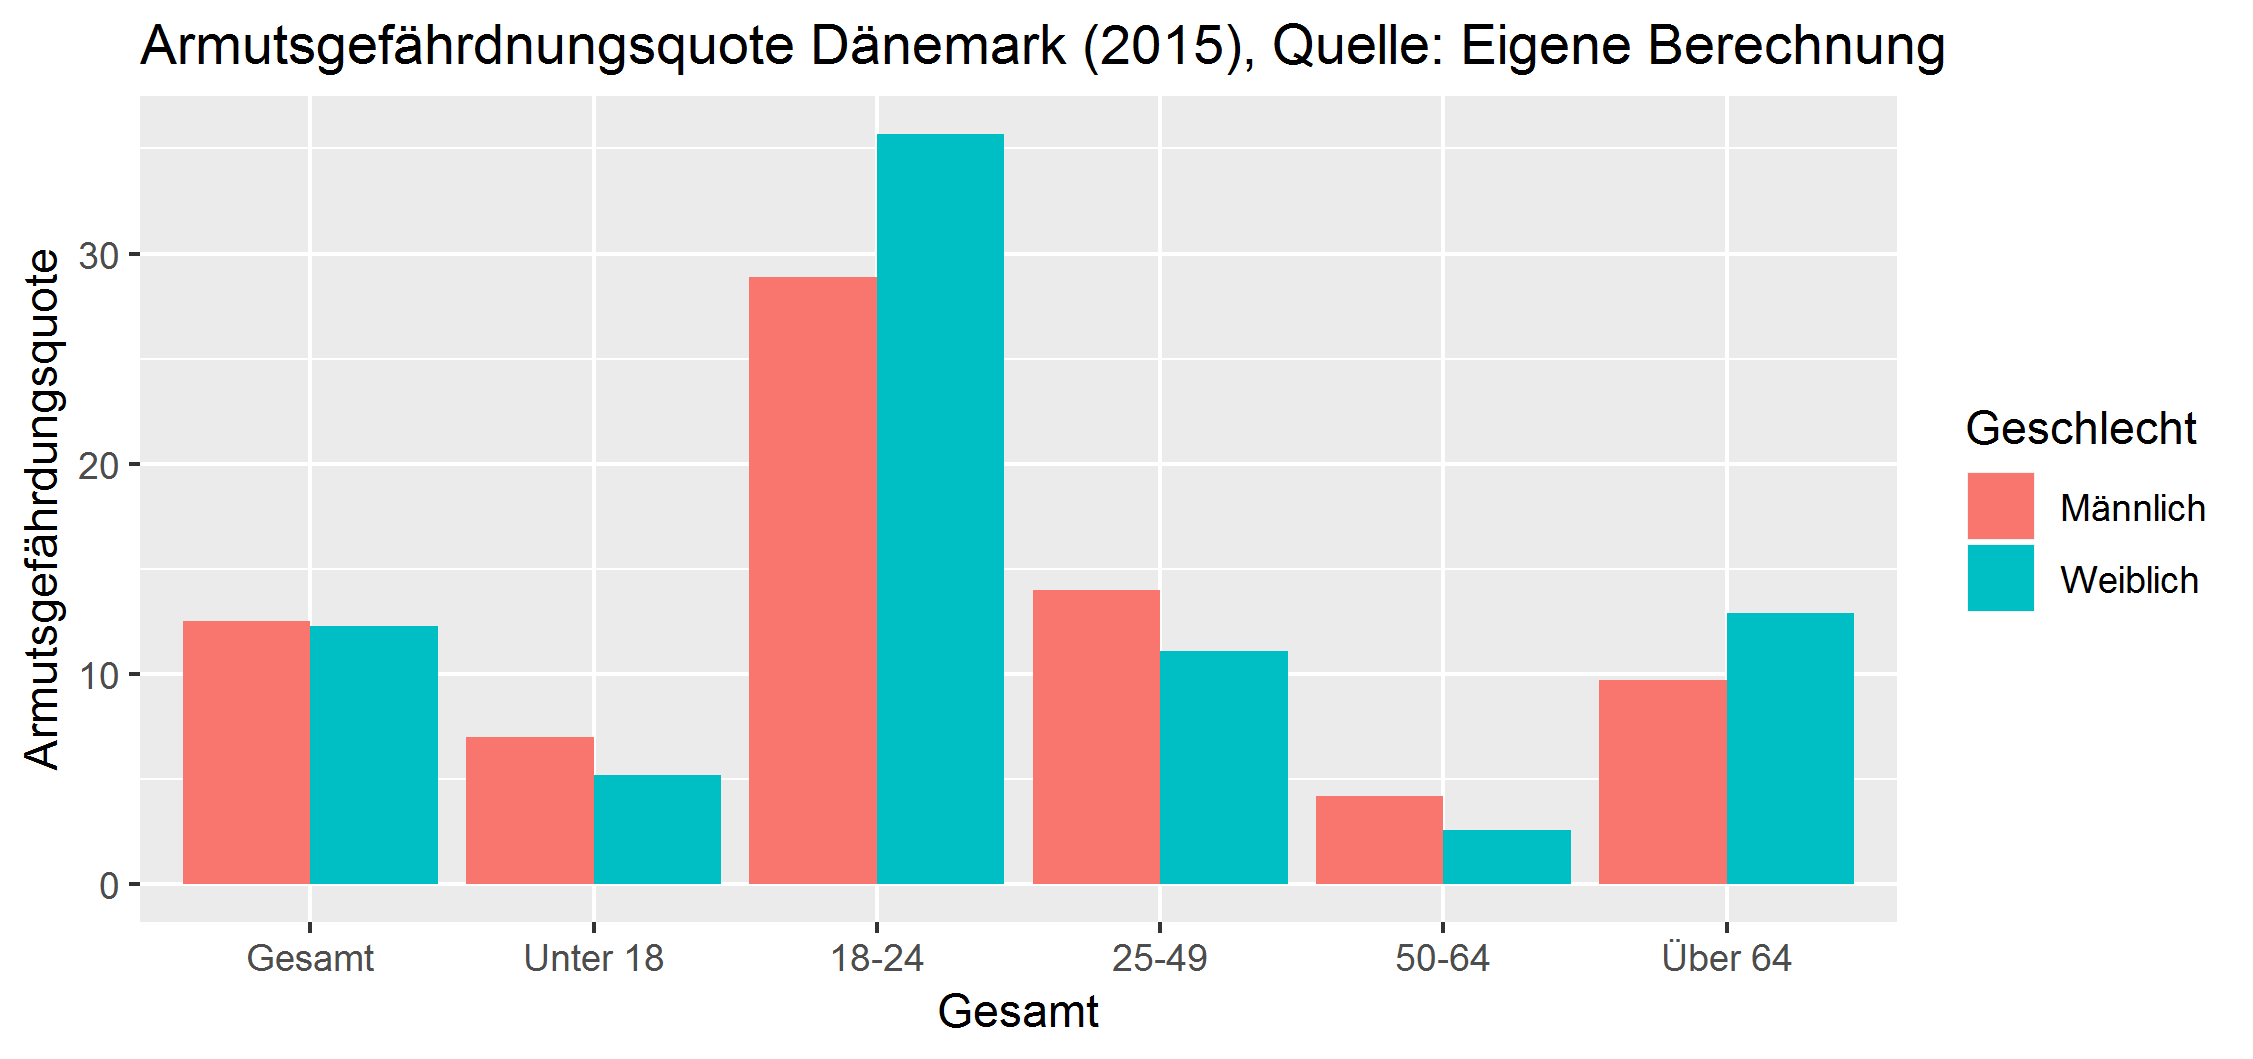
\includegraphics[width=0.90000\textwidth]{img/arpr_barplot.png}
\caption{Armutsgefährdungsquote 2015}
\end{figure}

Um einen besseren Eindruck davon zu gewinnen, welche Personengruppen
besonders von Armut gefährdet sind, wurden außerdem
Armutsgefähdrungsquoten nach Alter und Geschlecht für 2015 berechnet.
Die Grafik zeigt die Ergebnisse dieser Aufschlüsselung und im Anhang
findet sich eine Tabelle mit den exakten Werten. Aus der Aufschlüsselung
ist ersichtlich, dass insbesondere Personen zwischen 18 und 24 Jahren
von Armut gefährdet sind. Nach unseren Berechnungen ist dies bei 28,9
der Frauen und 35,7\% der Männer im Alter zwischen 18 und 24 Jahren der
Fall. Hierbei ist festzuhalten dass diese Kennzahlen mit äquivalisierten
Einkommen berechnet wurden, wodurch in einem Haushalt entweder alle
Personen Armutsgefährdet sind oder niemand. Eurostat verwendet hierfür
Personeneinkommen. Bei dieser vorgehensweise können auch einzelne
Personen in einem Haushalt als armutsgefährdet eingestuft werden. Dieser
methodische Unterschied spiegelt sich auch in den Resultaten wider.
Besonders groß ist er bei Männern zwischen 18 und 24 Jahren; die von
Eurostat berechnete Armutsgefährdungsquote beträgt für diese Gruppe
36,3\%. (Daten kontrollieren!!!)

Die Zerlegung der Armutsgefährdungsquote nach Geschlecht zeigt folgendes
Bild:

Die Tabelle zeigt welcher Prozentsatz an Armutsgefährdeten nach den
beide Berechnungsmethoden weiblich, bzw. männlich ist. Auch hier ist ein
klarer Unterschied zwischen P1 und P2 erkennbar. Nach P2 ist die
Mehrheit der Armutsgefährdeten weiblich, während das Ergbnis von P2
diesen Schluss nicht zulässt.

Diese Tabelle zeigt nur auf den ersten Blick ein uneindeutiges Bild.
Zwar ist je nach Berechnungsmethode eine Gruppe innerhalb der
Armutsgefährdeten in der Mehrheit, jedoch sind die
Unter-Dreißig-Jährigen in der Grundgesamtheit stark unterrepräsentiert.
Daraus können wir schließen, dass Unter-Dreißig-Jährige in Dänemark
besonders von Armut gefährdet sind.

\section{6 Conclusio}\label{conclusio}

Insgesamt zeigen sämtliche Ergebnisse die starke umverteilende Wirkung
des dänischen Transfer- und Steuersystems. Ohne diesen Mechanismus wären
die Einkommen in Dänemark deutlich ungleicher verteilt. Zusammenfassend
lässt sich sagen, dass die Ungleichheit in Dänemark grundsätzlich
niedrig, im speziellen Beobachtungszeitraum, 2004-2017, jedoch leicht
gestiegen ist. Dieses Ergebnis ist im Einklang mit dem aktuellen Stand
der Forschung und dem internationalen Trend (OECD 2016a, Causa, Nicolas
Ruiz, and Zuzana Smidova (2016)). Die genauen Ursachen für diese
Entwicklung lassen sich mit den vorliegenden Daten vermutlich nicht
identifizieren. Fest steht jedoch, dass die schrittweise Verschärfung
der Bestimmungen zur Arbeitslosenunterstützung und damit der Rückgang
der BezieherInnen von Arbeitslosenunterstützung mit einem Anstieg an
SozialhilfeempfängerInnen und FrühpensionistInnen einherging (Gaard
2005, OECD (2016a)). Für uns lässt sich daraus schließen, dass das
Flexicurity-System Dänemarks, das Problem der Arbeitslosigkeit nur
oberflächlich zu lösen scheint.

Des weiteren konnten wir einen Anstieg der Armutsgefährungsquote in
Dänemark über den Beobachtungszeitraum feststellen, wobei Frauen und
Unter-Dreißig-Jährige in dieser Gruppe überrepräsentiert sind.
Anzumerken ist, dass dieser Effekt für Frauen nicht eindeutig ist. Auch
dieses Ergebnis deckt sich mit der bestehenden Literatur (OECD (2016b)).
Für die Agenda der EU, Europa2020, ist dies kein Fortschritt von
Dänemark im Bereich Armutsbekämpfung.

Anzumerken ist, dass die Ergebnisse dieser Arbeit nur einen kleinen Teil
der Einkommensungleichheit und Armut in Dänemark repräsentieren. Für
eine tiefergehende Analyse bedarf es noch mehr Forschung und zusätzliche
Daten. Besonders interessant wäre in diesem Sinne eine genauere
Betrachtung der Haushaltsstruktur.

\newpage

\section{Appendix}\label{appendix}

\textbf{Legende}

\begin{itemize}
\tightlist
\item
  \textbf{P1fakt:} Faktoreinkommen vor Steuern nach P1 Eurostat (eigene
  Berechnung)
\item
  \textbf{P1nat.:} Nationaleinkommen vor Steuern nach P1 Eurostat
  (eigene Berechnung)
\item
  \textbf{P1verf.:} Verfügbares Einkommen nach Steuern nach P1 Eurostat
  (eigene Berechnung)
\item
  \textbf{P2fakt.:} Faktoreinkommen vor Steuern nach P2 wid.world
  (eigene Berechnung)
\item
  \textbf{P2nat.:} Nationaleinkommen vor Steuern nach P2 wid.world
  (eigene Berechnung)
\item
  \textbf{P2verf.:} Verfügbares Einkommen nach Steuern nach P2 wid.world
  (eigene Berechnung)
\item
  \textbf{ESfakt.:} Eurostat Faktoreinkommen vor Steuern
\item
  \textbf{ESverf.:} Eurostat verfügbares Einkommen nach Steuern
\end{itemize}

~

\textbf{Gesamtübersichten der Indikatoren}

\begin{longtable}[]{@{}rrrrrrrr@{}}
\caption{Gesamtübersicht Mittelwert}\tabularnewline
\toprule
Jahr & P1fakt. & P1nat. & P1verf. & P2fakt. & P2nat. & P2verf. &
ESverf.\tabularnewline
\midrule
\endfirsthead
\toprule
Jahr & P1fakt. & P1nat. & P1verf. & P2fakt. & P2nat. & P2verf. &
ESverf.\tabularnewline
\midrule
\endhead
2004 & 34430.34 & 40891.98 & 28370.61 & 32915.76 & 38678.16 & 27293.91 &
27250.30\tabularnewline
2005 & 34474.53 & 40681.39 & 28651.63 & 33033.01 & 38532.54 & 27482.93 &
27404.71\tabularnewline
2006 & 34915.35 & 41210.60 & 28964.12 & 33469.94 & 39112.04 & 27832.18 &
27760.69\tabularnewline
2007 & 36614.52 & 42788.87 & 30037.79 & 32767.63 & 37975.43 & 33077.26 &
28537.50\tabularnewline
2008 & 36455.49 & 42404.63 & 29727.99 & 32664.52 & 37697.24 & 32687.69 &
28541.67\tabularnewline
2009 & 36382.80 & 42570.60 & 29976.66 & 32939.52 & 38202.15 & 33342.34 &
28118.35\tabularnewline
2010 & 36123.19 & 42613.77 & 30575.51 & 32705.73 & 38206.55 & 33734.08 &
28602.55\tabularnewline
2011 & 36733.95 & 43568.14 & 31416.40 & 33424.57 & 39197.48 & 34724.54 &
30379.92\tabularnewline
2012 & 35532.70 & 42582.28 & 30931.32 & 33039.80 & 39163.04 & 34834.15 &
30020.22\tabularnewline
2013 & 36410.88 & 43735.41 & 31577.54 & 34227.54 & 40682.65 & 36100.98 &
30263.58\tabularnewline
2014 & 37655.67 & 45537.10 & 32676.44 & 36375.47 & 43379.57 & 31693.98 &
31170.34\tabularnewline
2015 & 38132.84 & 46178.73 & 33226.56 & 36793.45 & 43959.14 & 32104.97 &
31518.00\tabularnewline
2016 & 39909.14 & 47567.60 & 33624.55 & 38451.81 & 45292.76 & 32772.00 &
32141.00\tabularnewline
2017 & 39785.66 & 47722.42 & 33775.70 & 38356.84 & 45432.31 & 32784.68 &
32435.21\tabularnewline
\bottomrule
\end{longtable}

\begin{longtable}[]{@{}rrrrrrrr@{}}
\caption{Gesamtübersicht Median}\tabularnewline
\toprule
Jahr & P1fakt. & P1nat. & P1verf. & P2fakt. & P2nat. & P2verf. &
ESverf.\tabularnewline
\midrule
\endfirsthead
\toprule
Jahr & P1fakt. & P1nat. & P1verf. & P2fakt. & P2nat. & P2verf. &
ESverf.\tabularnewline
\midrule
\endhead
2004 & 33157.57 & 37304.94 & 26361.07 & 32930.26 & 35231.47 & 24137.49 &
25419.16\tabularnewline
2005 & 33386.58 & 37659.82 & 27127.42 & 33598.70 & 35976.64 & 24701.63 &
26028.24\tabularnewline
2006 & 33750.79 & 38127.54 & 27321.69 & 33842.41 & 36321.14 & 24928.25 &
26200.00\tabularnewline
2007 & 34847.34 & 38895.62 & 27803.14 & 32228.55 & 35254.31 & 30140.08 &
26523.86\tabularnewline
2008 & 34428.25 & 37702.56 & 27280.28 & 31938.67 & 34690.18 & 29517.02 &
26492.32\tabularnewline
2009 & 35616.96 & 39030.71 & 28248.49 & 32858.34 & 35807.18 & 30724.11 &
27175.90\tabularnewline
2010 & 34407.02 & 38749.23 & 28508.38 & 33387.50 & 36204.45 & 31416.38 &
27277.36\tabularnewline
2011 & 34849.23 & 39571.97 & 28865.47 & 32876.25 & 36828.55 & 31857.22 &
27892.34\tabularnewline
2012 & 33096.32 & 38489.05 & 28229.03 & 32527.04 & 36583.24 & 31593.33 &
27486.35\tabularnewline
2013 & 33581.99 & 39159.14 & 28470.82 & 33880.42 & 37709.14 & 32559.22 &
27609.66\tabularnewline
2014 & 33791.30 & 39838.12 & 29256.93 & 34255.25 & 38823.39 & 27380.34 &
27916.83\tabularnewline
2015 & 35097.38 & 40867.56 & 29862.23 & 35880.45 & 39682.86 & 27911.45 &
28364.00\tabularnewline
2016 & 35063.49 & 41051.65 & 30068.52 & 36722.67 & 40376.15 & 28315.64 &
28665.00\tabularnewline
2017 & 35571.66 & 42095.37 & 30307.75 & 36574.66 & 40879.46 & 28565.74 &
29063.30\tabularnewline
\bottomrule
\end{longtable}

\begin{longtable}[]{@{}rrrrrrrrr@{}}
\caption{Gesamtübersicht Gini-Koeffizienten}\tabularnewline
\toprule
Jahr & P1fakt. & P1nat. & P1verf. & P2fakt. & P2nat. & P2verf. & ESfakt.
& ESverf.\tabularnewline
\midrule
\endfirsthead
\toprule
Jahr & P1fakt. & P1nat. & P1verf. & P2fakt. & P2nat. & P2verf. & ESfakt.
& ESverf.\tabularnewline
\midrule
\endhead
2004 & 0.44 & 0.31 & 0.23 & 0.47 & 0.34 & 0.32 & 0.45 &
0.24\tabularnewline
2005 & 0.43 & 0.31 & 0.23 & 0.47 & 0.34 & 0.31 & 0.44 &
0.24\tabularnewline
2006 & 0.43 & 0.31 & 0.23 & 0.46 & 0.34 & 0.31 & 0.44 &
0.24\tabularnewline
2007 & 0.44 & 0.32 & 0.24 & 0.49 & 0.38 & 0.34 & 0.45 &
0.25\tabularnewline
2008 & 0.45 & 0.33 & 0.25 & 0.50 & 0.39 & 0.35 & 0.46 &
0.25\tabularnewline
2009 & 0.44 & 0.32 & 0.23 & 0.49 & 0.38 & 0.34 & 0.59 &
0.27\tabularnewline
2010 & 0.44 & 0.33 & 0.25 & 0.49 & 0.37 & 0.34 & 0.51 &
0.27\tabularnewline
2011 & 0.46 & 0.34 & 0.26 & 0.51 & 0.39 & 0.35 & 0.51 &
0.27\tabularnewline
2012 & 0.46 & 0.34 & 0.26 & 0.50 & 0.38 & 0.34 & 0.51 &
0.26\tabularnewline
2013 & 0.46 & 0.34 & 0.26 & 0.51 & 0.38 & 0.34 & 0.51 &
0.27\tabularnewline
2014 & 0.48 & 0.35 & 0.27 & 0.51 & 0.39 & 0.35 & 0.53 &
0.28\tabularnewline
2015 & 0.47 & 0.34 & 0.27 & 0.50 & 0.37 & 0.35 & 0.52 &
0.27\tabularnewline
2016 & 0.48 & 0.35 & 0.27 & 0.51 & 0.38 & 0.36 & 0.51 &
0.28\tabularnewline
2017 & 0.47 & 0.34 & 0.27 & 0.51 & 0.38 & 0.35 & 0.50 &
0.28\tabularnewline
\bottomrule
\end{longtable}

\begin{longtable}[]{@{}rrrrrrrr@{}}
\caption{Gesamtübersicht P80/P20 Verhältnis}\tabularnewline
\toprule
Jahr & P1fakt. & P1nat. & P1verf. & P2fakt. & P2nat. & P2verf. &
ESverf.\tabularnewline
\midrule
\endfirsthead
\toprule
Jahr & P1fakt. & P1nat. & P1verf. & P2fakt. & P2nat. & P2verf. &
ESverf.\tabularnewline
\midrule
\endhead
2004 & 45.85 & 5.54 & 3.19 & 86.91 & 7.14 & 5.39 & 3.4\tabularnewline
2005 & 49.39 & 5.61 & 3.16 & 102.86 & 7.45 & 5.25 & 3.5\tabularnewline
2006 & 48.21 & 5.42 & 3.22 & 100.37 & 7.03 & 5.21 & 3.4\tabularnewline
2007 & 51.50 & 5.82 & 3.39 & 214.24 & 10.47 & 6.93 & 3.7\tabularnewline
2008 & 55.33 & 6.21 & 3.49 & 192.43 & 11.03 & 7.12 & 3.6\tabularnewline
2009 & 55.01 & 6.03 & 3.36 & 202.51 & 10.48 & 6.90 & 4.6\tabularnewline
2010 & 58.63 & 6.17 & 3.58 & 230.76 & 10.80 & 7.18 & 4.4\tabularnewline
2011 & 72.15 & 6.63 & 3.77 & 282.05 & 12.19 & 7.56 & 4.0\tabularnewline
2012 & 79.19 & 6.80 & 3.77 & 269.66 & 11.04 & 6.85 & 3.9\tabularnewline
2013 & 64.09 & 6.53 & 3.69 & 227.37 & 10.74 & 6.77 & 4.0\tabularnewline
2014 & 79.43 & 7.40 & 3.99 & 157.06 & 10.18 & 6.45 & 4.1\tabularnewline
2015 & 67.33 & 6.67 & 3.86 & 141.34 & 9.03 & 6.35 & 4.1\tabularnewline
2016 & 58.40 & 6.80 & 3.85 & 130.63 & 9.39 & 6.61 & 4.1\tabularnewline
2017 & 67.42 & 6.74 & 3.92 & 145.39 & 9.31 & 6.74 & 4.1\tabularnewline
\bottomrule
\end{longtable}

\begin{longtable}[]{@{}rrrrrrrr@{}}
\caption{Gesamtübersicht Top 10\% Anteil}\tabularnewline
\toprule
Jahr & P1fakt. & P1nat. & P1verf. & P2fakt. & P2nat. & P2verf. &
ESverf.\tabularnewline
\midrule
\endfirsthead
\toprule
Jahr & P1fakt. & P1nat. & P1verf. & P2fakt. & P2nat. & P2verf. &
ESverf.\tabularnewline
\midrule
\endhead
2004 & 0.27 & 0.23 & 0.20 & 0.29 & 0.25 & 0.25 & 0.20\tabularnewline
2005 & 0.26 & 0.23 & 0.19 & 0.28 & 0.25 & 0.24 & 0.20\tabularnewline
2006 & 0.26 & 0.23 & 0.20 & 0.28 & 0.24 & 0.24 & 0.20\tabularnewline
2007 & 0.28 & 0.24 & 0.21 & 0.30 & 0.26 & 0.25 & 0.21\tabularnewline
2008 & 0.28 & 0.25 & 0.21 & 0.30 & 0.27 & 0.25 & 0.21\tabularnewline
2009 & 0.27 & 0.24 & 0.20 & 0.29 & 0.25 & 0.24 & 0.20\tabularnewline
2010 & 0.27 & 0.24 & 0.21 & 0.28 & 0.25 & 0.24 & 0.21\tabularnewline
2011 & 0.28 & 0.25 & 0.22 & 0.30 & 0.27 & 0.25 & 0.22\tabularnewline
2012 & 0.29 & 0.25 & 0.22 & 0.30 & 0.26 & 0.25 & 0.22\tabularnewline
2013 & 0.29 & 0.25 & 0.22 & 0.31 & 0.27 & 0.26 & 0.22\tabularnewline
2014 & 0.30 & 0.26 & 0.23 & 0.32 & 0.28 & 0.27 & 0.23\tabularnewline
2015 & 0.30 & 0.26 & 0.22 & 0.32 & 0.27 & 0.27 & 0.23\tabularnewline
2016 & 0.31 & 0.27 & 0.23 & 0.33 & 0.28 & 0.28 & 0.23\tabularnewline
2017 & 0.30 & 0.26 & 0.23 & 0.32 & 0.28 & 0.27 & 0.23\tabularnewline
\bottomrule
\end{longtable}

\begin{longtable}[]{@{}rrrrrrrr@{}}
\caption{Gesamtübersicht Armutsgefährdungsquote}\tabularnewline
\toprule
Jahr & P1fakt. & P1nat. & P1verf. & P2fakt. & P2nat. & P2verf. &
ESverf.\tabularnewline
\midrule
\endfirsthead
\toprule
Jahr & P1fakt. & P1nat. & P1verf. & P2fakt. & P2nat. & P2verf. &
ESverf.\tabularnewline
\midrule
\endhead
2004 & 32.71 & 21.08 & 10.59 & 37.09 & 24.09 & 19.92 &
10.9\tabularnewline
2005 & 32.50 & 21.95 & 11.33 & 37.21 & 25.21 & 19.55 &
11.8\tabularnewline
2006 & 32.19 & 21.36 & 11.60 & 37.01 & 25.20 & 19.73 &
11.7\tabularnewline
2007 & 32.09 & 21.75 & 11.72 & 38.90 & 28.91 & 23.53 &
11.7\tabularnewline
2008 & 32.72 & 22.01 & 11.90 & 38.75 & 29.10 & 23.21 &
11.8\tabularnewline
2009 & 32.68 & 23.08 & 12.49 & 39.10 & 29.70 & 24.17 &
13.1\tabularnewline
2010 & 32.90 & 22.61 & 12.75 & 39.48 & 29.69 & 24.05 &
13.3\tabularnewline
2011 & 33.54 & 22.13 & 13.11 & 39.65 & 29.29 & 24.82 &
12.1\tabularnewline
2012 & 34.23 & 22.35 & 13.15 & 40.01 & 28.97 & 23.88 &
12.0\tabularnewline
2013 & 34.43 & 21.39 & 11.76 & 40.66 & 28.43 & 24.06 &
11.9\tabularnewline
2014 & 34.04 & 20.92 & 12.33 & 38.77 & 26.51 & 22.18 &
12.1\tabularnewline
2015 & 33.72 & 20.99 & 12.38 & 39.00 & 26.36 & 22.04 &
12.2\tabularnewline
2016 & 33.61 & 20.09 & 12.04 & 39.43 & 26.68 & 23.13 &
11.9\tabularnewline
2017 & 33.94 & 20.82 & 12.54 & 39.12 & 26.75 & 23.19 &
12.4\tabularnewline
\bottomrule
\end{longtable}

\begin{longtable}[]{@{}rrll@{}}
\caption{Vergleich Armutsgefährdungsquote}\tabularnewline
\toprule
Eigene Berechnung & Eurostat & Geschlecht & Altersgruppe\tabularnewline
\midrule
\endfirsthead
\toprule
Eigene Berechnung & Eurostat & Geschlecht & Altersgruppe\tabularnewline
\midrule
\endhead
12.5 & 12.5 & Männlich & Gesamt\tabularnewline
12.3 & 11.9 & Weiblich & Gesamt\tabularnewline
7.0 & 10.1 & Männlich & Unter 18\tabularnewline
5.2 & 10.6 & Weiblich & Unter 18\tabularnewline
28.9 & 36.3 & Männlich & 18-24\tabularnewline
35.7 & 38.7 & Weiblich & 18-24\tabularnewline
14.0 & 13.5 & Männlich & 25-49\tabularnewline
11.1 & 11.2 & Weiblich & 25-49\tabularnewline
4.2 & 6.3 & Männlich & 50-64\tabularnewline
2.6 & 4.4 & Weiblich & 50-64\tabularnewline
9.7 & 8.0 & Männlich & Über 64\tabularnewline
12.9 & 10.0 & Weiblich & Über 64\tabularnewline
\bottomrule
\end{longtable}

\newpage

\section{Literatur}\label{literatur}

\hypertarget{refs}{}
\hypertarget{ref-atkinson2016long}{}
Atkinson, Jakob Egholt, Anthony B und Søgaard. 2016. ``The Long-Run
History of Income Inequality in Denmark.'' \emph{The Scandinavian
Journal of Economics} 118 (2). Wiley Online Library: 264--91.

\hypertarget{ref-bammer2003armut}{}
Bammer, Andreas. 2003. ``„Armut in Der Alltagssprache: Etymologie Und
Phänomenologie Des Begriffs.'' \emph{Böhm, Renate/Buggler,
Robert/Mautner, Josef (Hg.)(2003): Arbeiten Am Begriff Der Armut},
19--25.

\hypertarget{ref-bjorklund2000going}{}
Björklund, Anders. 2000. ``Going Different Ways: Labour Market Policy in
Denmark and Sweden.'' \emph{Why Deregulate Labour Markets}, 148--80.

\hypertarget{ref-Jespersen}{}
Bohn-Jespersen, und Mogensen, H. 2018. ``While the Sun Is Shining,
Prepare for a Rainy Day.'' \emph{Danmarks Nationalbank, Copenhagen},
Analysis, No.16.

\hypertarget{ref-causa2016inequality}{}
Causa, Orsetta, Mikkel Hermansen und Nicolas Ruiz, and Caroline Klein
und Zuzana Smidova. 2016. ``Inequality in Denmark Through the Looking
Glass,'' no. 1341.
doi:\href{https://doi.org/https://doi.org/https://doi.org/10.1787/5jln041vm6tg-en}{https://doi.org/https://doi.org/10.1787/5jln041vm6tg-en}.

\hypertarget{ref-cawistat}{}
Danmarks Statistik. 2014. ``Web-Interviewing for the Danish Eu-Silc -
Our Experience.''

\hypertarget{ref-statdenm2}{}
---------. 2019a. ``How Has Denmark Managed Since the Finansial
Crisis.'' Accessed January 2.
\url{http://www.nationalbanken.dk/en/publications/themes/Pages/How-has-Denmark-managed-since-the-finansial-crisis.aspx}.

\hypertarget{ref-statdenm}{}
---------. 2019b. ``Income Statistics Comparability.'' Accessed January
2.
\url{https://www.dst.dk/en/Statistik/dokumentation/documentationofstatistics/income-statistics/comparability}.

\hypertarget{ref-denmark2020}{}
Dänische Regierung. 2010. ``Denmark 2020 - Knowledge, Growth,
Prosperity, Welfare.''
\url{http://www.stm.dk/publikationer/arbprog_10_uk/Denmark_2020_knowledge_growth_prosperity_welfare.pdf}.

\hypertarget{ref-danski}{}
Dänischer Wirtschaftsrat. 2019. ``Danish Economy Fall 2016. English
Summary, P. 335f.'' Accessed February 15.
\url{https://dors.dk/vismandsrapporter/dansk-oekonomi-efteraar-2016}.

\hypertarget{ref-integr}{}
Dänisches Ministerium für Flüchtlinge, Einwanderer und Integration.
2017. ``International Migration -- Denmark. Report to the Oecd.''

\hypertarget{ref-eudenm}{}
Europäische Kommission. 2019. ``Europe 2020 Targets: Statistics and
Indicators for Denmark.'' Accessed February 15.
\url{https://ec.europa.eu/info/business-economy-euro/economic-and-fiscal-policy-coordination/eu-economic-governance-monitoring-prevention-correction/european-semester/european-semester-your-country/denmark}.

\hypertarget{ref-silcmanual}{}
Eurostat. 2013a. \emph{Description of Target Variables: Cross-Sectional
and Longitudinal}.

\hypertarget{ref-cawi}{}
---------. 2013b. ``Working Group Meeting `Statistics on Living
Conditions' 11-13 June.'' Eurostat Luxembourg, JMO Building, Room M4:
Eurostat.

\hypertarget{ref-eurostatweb}{}
---------. 2019. ``Statistik Der Europäischen Union über Einkommen Und
Lebensbedingungen (Eu-Silc).'' Accessed January 2.
\url{https://ec.europa.eu/eurostat/web/microdata/european-union-statistics-on-income-and-living-conditions}.

\hypertarget{ref-gaard2005two}{}
Gaard, Mads, Sflren und Kieler. 2005. ``Two Decades of Structural Reform
in Denmark: A Review.'' \emph{Danish Ministry of Finance Working Paper},
no. 16.

\hypertarget{ref-gallen2019labor}{}
Gallen, Rune V und Vejlin, Yana und Lesner. 2019. ``The Labor Market
Gender Gap in Denmark: Sorting Out the Past 30 Years.'' \emph{Labour
Economics} 56. Elsevier: 58--67.

\hypertarget{ref-joyce2018inspiration}{}
Joyce, Patrick. 2018. ``Inspiration for Integration. Labour Market
Policies for Refugees in Five Northern European Countries.'' The Ratio
Institute.

\hypertarget{ref-oecd2008growing}{}
OECD. 2008. \emph{Growing Unequal?: Income Distribution and Poverty in
Oecd Countries}.

\hypertarget{ref-oecd2015together}{}
---------. 2015. \emph{In It Together: Why Less Inequality Benefits
All}. OECD publishing.

\hypertarget{ref-oecd2016survey}{}
---------. 2016a. \emph{OECD Economic Surveys: Denmark 2016}.
doi:\href{https://doi.org/https://doi.org/https://doi.org/10.1787/eco_surveys-dnk-2016-en}{https://doi.org/https://doi.org/10.1787/eco\_surveys-dnk-2016-en}.

\hypertarget{ref-oecd2016society}{}
---------. 2016b. \emph{Society at a Glance 2016}.
doi:\href{https://doi.org/https://doi.org/https://doi.org/10.1787/9789264261488-en}{https://doi.org/https://doi.org/10.1787/9789264261488-en}.

\hypertarget{ref-oecd2019survey}{}
---------. 2019a. \emph{OECD Economic Surveys: Denmark 2019}.
\url{https://read.oecd-ilibrary.org/economics/oecd-economic-surveys-denmark-2019_eco_surveys-dnk-2019-en}.

\hypertarget{ref-oecdpop}{}
---------. 2019b. ``OECD Data - Population.'' Accessed February 15.
\url{https://data.oecd.org/pop/population.htm}.

\hypertarget{ref-robling2018demographic}{}
Robling, Jon Kristian, Per-Olof und Pareliussen. 2018. ``Demographic
Change and Inequality Trends in the Nordic Countries.'' \emph{Nordic
Economic Policy Review}, 136--66.

\hypertarget{ref-europe2020}{}
Statistisches Amt Europäische Kommission. 2016. ``Smarter, Greener, More
Inclusive?: Indicators to Support the Europe 2020 Strategy.''
Publications Office of the European Union.

\hypertarget{ref-Menschenr}{}
Vereine Nationen. 1948. ``Allgemeine Erklärung Der Menschenrechte.''
\url{http://www.un.org/depts/german/menschenrechte/aemr.pdf}.


\end{document}
